\documentclass[12pt,oneside,openany]{memoir}

\usepackage{fontspec}
\setmainfont{Latin Modern Roman}
\setsansfont{Latin Modern Sans}
\setmonofont{Latin Modern Mono}
% The base image does not ship babel-danish. XeLaTeX still handles the
% UTF-8 Danish text correctly; hyphenation remains conservative and readable.
\usepackage[english]{babel}
\usepackage{microtype}
\usepackage{geometry}
\geometry{paperwidth=17cm,paperheight=24cm,inner=2.05cm,outer=1.75cm,top=1.85cm,bottom=2.0cm,headheight=16pt,headsep=0.45cm,footskip=0.8cm}
\special{papersize=17cm,24cm}
% memoir emulates setspace; a modest line spread keeps the larger type airy.
\linespread{1.08}
\usepackage{amsmath,amssymb}
\usepackage{array,booktabs,longtable,tabularx,ragged2e}
\usepackage{enumitem}
\usepackage{graphicx}
\usepackage{tikz}
\usetikzlibrary{arrows.meta,positioning,calc,fit,shapes.geometric}
\usepackage{xcolor}
\usepackage[most]{tcolorbox}
\usepackage{csquotes}
\usepackage{xurl}
\usepackage{natbib}
\usepackage{fancyhdr}
\usepackage{hyperref}
\usepackage{bookmark}

\definecolor{ink}{HTML}{172B4D}
\definecolor{accent}{HTML}{197C8C}
\definecolor{warm}{HTML}{C9783B}
\definecolor{paper}{HTML}{F7F8FA}
\definecolor{muted}{HTML}{5E6B7A}
\definecolor{line}{HTML}{D8E0E8}
\definecolor{softblue}{HTML}{EAF3F6}
\definecolor{softwarm}{HTML}{FBF0E8}
\definecolor{softgray}{HTML}{F1F3F5}

\hypersetup{
  colorlinks=true,
  linkcolor=ink,
  citecolor=accent,
  urlcolor=accent,
  pdftitle={Jura fra bunden},
  pdfauthor={Scott Brodie Forsyth},
  pdfsubject={Introduktion til dansk ret og juridisk metode}
}

\setsecnumdepth{subsection}
\settocdepth{subsection}
\setlength{\parindent}{0pt}
\setlength{\parskip}{0.55em}
\setlength{\emergencystretch}{3em}
\setlist[itemize]{leftmargin=1.35em,itemsep=0.2em,topsep=0.25em}
\setlist[enumerate]{leftmargin=1.55em,itemsep=0.25em,topsep=0.25em}

\makeatletter
\makechapterstyle{cleanlaw}{%
  \renewcommand{\chapnamefont}{\sffamily\bfseries\color{accent}\large}
  \renewcommand{\chapnumfont}{\sffamily\bfseries\color{accent}\fontsize{42}{42}\selectfont}
  \renewcommand{\chaptitlefont}{\sffamily\bfseries\color{ink}\Huge}
  \renewcommand{\printchaptername}{\chapnamefont\@chapapp}
  \renewcommand{\printchapternum}{\chapnumfont\thechapter}
  \renewcommand{\afterchapternum}{\par\vskip 6pt}
  \renewcommand{\printchaptertitle}[1]{\chaptitlefont ##1\par}
  \setlength{\beforechapskip}{0pt}
  \setlength{\afterchapskip}{30pt}
}
\makeatother
\chapterstyle{cleanlaw}
\setsecheadstyle{\Large\sffamily\bfseries\color{ink}}
\setsubsecheadstyle{\large\sffamily\bfseries\color{accent}}
\setsubsubsecheadstyle{\normalsize\sffamily\bfseries\color{ink}}

\newtcolorbox{keybox}{
  enhanced,breakable,boxrule=0pt,frame hidden,
  colback=softblue,coltext=ink,left=10pt,right=10pt,top=8pt,bottom=8pt,
  borderline west={3pt}{0pt}{accent},before skip=8pt,after skip=12pt
}
\newtcolorbox{examplebox}{
  enhanced,breakable,boxrule=0.5pt,colframe=line,colback=paper,
  coltext=ink,left=10pt,right=10pt,top=8pt,bottom=8pt,
  before skip=8pt,after skip=12pt
}
\newtcolorbox{warningbox}{
  enhanced,breakable,boxrule=0pt,frame hidden,
  colback=softwarm,coltext=ink,left=10pt,right=10pt,top=8pt,bottom=8pt,
  borderline west={3pt}{0pt}{warm},before skip=8pt,after skip=12pt
}
\newtcolorbox{methodbox}{
  enhanced,breakable,boxrule=0.5pt,colframe=accent,colback=white,
  coltext=ink,left=10pt,right=10pt,top=8pt,bottom=8pt,
  before skip=8pt,after skip=12pt
}
\newcommand{\term}[1]{\textbf{#1}}
\newcommand{\law}[1]{\textsc{#1}}
\newcommand{\important}[1]{\textbf{\color{accent}#1}}
\newcommand{\chapterlead}[1]{\begin{keybox}\textbf{Hovedidé.} #1\end{keybox}}
\newcommand{\question}[1]{\begin{examplebox}\textbf{Tænk over det.} #1\end{examplebox}}
\newcommand{\practice}[1]{\begin{methodbox}\textbf{Arbejdsgang.} #1\end{methodbox}}
\newcommand{\caution}[1]{\begin{warningbox}\textbf{Pas på.} #1\end{warningbox}}

\pagestyle{fancy}
\fancyhf{}
\fancyhead[R]{\sffamily\small\color{muted}\rightmark}
\fancyhead[L]{\sffamily\small\color{muted}\thepage}
\renewcommand{\chaptermark}[1]{\markright{#1}}
\renewcommand{\headrulewidth}{0pt}
\fancypagestyle{plain}{%
  \fancyhf{}\fancyfoot[C]{\sffamily\small\color{muted}\thepage}\renewcommand{\headrulewidth}{0pt}}

\begin{document}

\clearpage
\thispagestyle{empty}

\begin{tikzpicture}[remember picture,overlay]
  \fill[ink] (current page.south west) rectangle ([xshift=17cm,yshift=28cm]current page.south west);
  \fill[accent] (current page.south west) rectangle ([xshift=2.35cm,yshift=28cm]current page.south west);
  \fill[warm] ([yshift=27.72cm]current page.south west) rectangle ([xshift=17cm,yshift=28cm]current page.south west);
  \node[anchor=west,text=white!75,font=\sffamily\fontsize{8.5}{10}\selectfont] at ([xshift=2.05cm,yshift=20.35cm]current page.south west) {EN INTRODUKTIONSBOG · DANSK RET};
  \node[anchor=west,text=white,font=\sffamily\bfseries\fontsize{34}{38}\selectfont] at ([xshift=2.05cm,yshift=16.7cm]current page.south west) {Jura};
  \node[anchor=west,text=white,font=\sffamily\bfseries\fontsize{34}{38}\selectfont] at ([xshift=2.05cm,yshift=15.55cm]current page.south west) {fra bunden};
  \node[anchor=west,text=white!80,text width=10.8cm,align=left,font=\sffamily\large] at ([xshift=2.05cm,yshift=14.25cm]current page.south west) {En tilgængelig introduktion til juridisk tænkning og dansk ret};
  \draw[warm,line width=1.2pt] ([xshift=2.05cm,yshift=13.2cm]current page.south west) -- ([xshift=6.7cm,yshift=13.2cm]current page.south west);
  \node[anchor=west,text=white,font=\sffamily\fontsize{8.5}{10}\selectfont] at ([xshift=2.05cm,yshift=5.25cm]current page.south west) {Scott Brodie Forsyth};
  \node[anchor=west,text=white!65,font=\sffamily\fontsize{8}{9.5}\selectfont] at ([xshift=2.05cm,yshift=4.7cm]current page.south west) {Udgave 1.0 · 15. juli 2026};
\end{tikzpicture}
\clearpage

\frontmatter
\chapter*{Titel og formål}
\addcontentsline{toc}{chapter}{Titel og formål}
\thispagestyle{empty}
\vspace*{1.2cm}
{\sffamily\bfseries\Huge Jura fra bunden\par}
\vspace{0.4cm}
{\Large En introduktionsbog til juridisk tænkning og dansk ret\par}
\vspace{1.3cm}
Denne bog forklarer, hvordan man går fra et hverdagsproblem til et juridisk spørgsmål, hvordan man finder de relevante regler, og hvordan man argumenterer ansvarligt for en konklusion.

Den er skrevet med dansk ret som udgangspunkt. EU-retten, Den Europæiske Menneskerettighedskonvention og digitale regler behandles, hvor de er nødvendige for at forstå den ret, der møder mennesker, virksomheder og myndigheder i Danmark.

\vfill
\begin{keybox}
\textbf{Udgave 1.0 · 15. juli 2026}\par
Bogen er introduktionsstof, ikke konkret juridisk rådgivning. Retstilstanden ændrer sig, og en konkret sag kræver altid kontrol af den gældende lovtekst, praksis og eventuelt professionel rådgivning.
\end{keybox}
\clearpage

\chapter*{Forord}
\addcontentsline{toc}{chapter}{Forord}
Jura kan på afstand ligne en samling paragraffer, som kun jurister kan læse. På tæt hold er jura imidlertid en bestemt måde at stille spørgsmål på. Hvem har kompetence? Hvilken regel gælder? Hvilke fakta kan bevises? Hvilke hensyn må indgå? Hvad følger der af reglen, og hvad er kun en rimelig mavefornemmelse?

Bogen begynder derfor ikke med at forudsætte, at læseren allerede kan juridiske ord. Først beskrives idéen i almindeligt sprog. Derefter introduceres begrebet, den juridiske struktur og de typiske undtagelser. Det er vigtigt, fordi juridisk præcision ikke opstår ved at bruge mange fremmede ord. Den opstår ved at holde regler, fakta, fortolkning og vurdering adskilt.

Bogens eksempler er konstruerede, medmindre andet er angivet. De skal træne læserens metode, ikke give et færdigt svar på en virkelig sag. En bog kan lære dig at læse en regel og opdage de relevante spørgsmål; den kan ikke på forhånd kende alle dokumenter, tidsfrister, beviser og særlige regler i din konkrete situation.

\vspace{1em}
\begin{flushright}
Scott Brodie Forsyth\\
15. juli 2026
\end{flushright}

\chapter*{Sådan bruger du bogen}
\addcontentsline{toc}{chapter}{Sådan bruger du bogen}
Hvert kapitel følger den samme rytme:
\begin{enumerate}
  \item en intuitiv forklaring af problemet,
  \item de juridiske begreber og deres afgrænsning,
  \item en metode til at arbejde med spørgsmålet,
  \item et eller flere eksempler, og
  \item korte øvelser, der tvinger dig til at skelne mellem relevante og irrelevante oplysninger.
\end{enumerate}

Når du møder en juridisk problemstilling, så brug denne korte kontrol:
\begin{enumerate}
  \item Hvad er den præcise konflikt eller beslutning?
  \item Hvem er parterne, og hvilken rolle har de?
  \item Hvilken myndighed eller domstol kan være kompetent?
  \item Hvilke faktiske oplysninger er sikre, usikre eller omstridte?
  \item Hvilke retskilder kan regulere situationen?
  \item Hvilke betingelser skal være opfyldt, før reglen får virkning?
  \item Hvilke retsfølger følger af en overtrædelse eller opfyldelse?
  \item Hvilke modargumenter og undtagelser skal behandles?
\end{enumerate}

\tableofcontents*

\mainmatter
\chapter{Hvad er ret?}

\chapterlead{Jura er samfundets organiserede måde at afgøre, hvad mennesker, virksomheder og myndigheder må, skal og kan gøre. Det juridiske svar afhænger ikke kun af, hvad der føles rimeligt, men af en metode, der forbinder autoritative kilder med dokumenterede fakta.}

\section{En hverdag uden juridiske ord}

Forestil dig, at du køber en computer på nettet. Den bliver leveret med en revne i skærmen. Sælgeren siger, at varen var i orden, da den forlod lageret. Du mener, at sælgeren må reparere eller omlevere den. Hvad er problemet?

I hverdagssprog kan man spørge: Hvem har ret? I jura må spørgsmålet gøres mere præcist:

\begin{itemize}
  \item Er der indgået en aftale, og hvad gik den ud på?
  \item Er computeren mangelfuld efter køberetten?
  \item Hvem skal bevise, hvornår skaden opstod?
  \item Hvilke krav kan køberen gøre gældende?
  \item Gælder der særlige regler, fordi køberen er forbruger?
  \item Hvilken tidsfrist og hvilken klagevej gælder?
\end{itemize}

Juridisk tænkning begynder altså med at omforme en fortælling til en række afgørelsesspørgsmål. En konflikt kan være følelsesmæssigt enkel og juridisk flerleddet. Omvendt kan en lang juridisk tekst løse et meget konkret problem.

\section{Ret, moral, politik og almindelig praksis}

Ordet ``ret'' bruges på flere måder. Vi kan mene et krav: ``Jeg har ret til at få pengene tilbage.'' Vi kan mene et system: ``Dansk ret siger ...'' Vi kan mene retfærdighed: ``Det er ikke retfærdigt.'' Disse udsagn hænger sammen, men de er ikke identiske.

En regel kan være juridisk gyldig, selv om mange mener, at den er dårlig eller uretfærdig. Det betyder ikke, at moral og politik er irrelevante. De kan påvirke lovgivning, fortolkning og udviklingen af principper. Men den juridiske analyse skal sige tydeligt, hvornår den beskriver gældende ret, og hvornår den argumenterer for, hvordan retten bør ændres.

\begin{examplebox}
\textbf{Tre forskellige udsagn.}

\emph{Juridisk:} ``Loven giver myndigheden adgang til at træffe afgørelsen.''

\emph{Moralsk:} ``Afgørelsen behandler borgeren urimeligt.''

\emph{Politisk:} ``Reglen bør ændres, så borgeren får større beskyttelse.''

Man kan fremsætte alle tre udsagn på én gang, men de bør ikke blandes sammen i samme konklusion.
\end{examplebox}

Retlige normer adskiller sig også fra skik og god praksis. En butik kan have en venlig kundepolitik, der går længere end loven. En branche kan have en fast fremgangsmåde, som kan få betydning som handelsbrug. Men en intern praksis er ikke automatisk en bindende regel. Spørgsmålet er, om den har en juridisk forankring, og hvilken rolle den spiller i den konkrete retskildekontekst.

\section{Hvad gør retten?}

Retssystemet har flere funktioner, som nogle gange trækker i forskellige retninger.

\begin{description}[style=nextline,leftmargin=0pt,labelindent=0pt]
  \item[Koordinering] Regler gør det muligt at planlægge. En kontrakt, en ejendomsregistrering og en frist reducerer usikkerhed.
  \item[Konfliktløsning] Domstole og klageorganer kan afgøre, hvem der skal bære en byrde, når parterne ikke selv kan blive enige.
  \item[Begrænsning af magt] Forfatningsret, menneskerettigheder og forvaltningsret sætter rammer for offentlige indgreb.
  \item[Fordeling] Skatte-, social-, familie- og arbejdsret fordeler muligheder, byrder og risici.
  \item[Udtryk for fælles beslutninger] Lovgivning gør politiske prioriteringer til generelle regler, der skal kunne anvendes på mange situationer.
  \item[Legitimering] Et offentligt indgreb fremstår mere legitimt, når det er truffet af rette organ efter en gennemsigtig procedure og med mulighed for kontrol.
\end{description}

Det er derfor for snævert at tænke på jura som straf. Straf er kun én del af retssystemet. De fleste juridiske spørgsmål handler om kompetence, aftaler, myndighedsafgørelser, erstatning, ejerskab, rettigheder eller procedurer.

\section{Retssystemet som institution}

En juridisk regel virker ikke alene. Den indgår i institutioner: Folketinget vedtager love, ministerier udsteder i visse tilfælde bekendtgørelser, myndigheder træffer afgørelser, domstolene fortolker og kontrollerer, og borgere og virksomheder tilpasser deres adfærd.

\begin{keybox}
En regel er ikke det samme som dens tekst. For at forstå reglen må man også undersøge, hvem der har udstedt den, hvilket område den gælder på, hvordan den fortolkes, og hvilken retsfølge den knytter til bestemte fakta.
\end{keybox}

Den britiske retsfilosof H. L. A. Hart beskrev retssystemet som en kombination af regler, der pålægger pligter, og regler, der bestemmer, hvordan regler skabes, ændres og anvendes \citep{hart}. Hans pointe kan omsættes til hverdagsniveau: Det er ikke nok at vide, at ``man skal gøre X''. Man må også vide, hvem der kan fastsætte X, hvordan man ændrer reglen, og hvem der afgør, om X er overtrådt.

Alf Ross lagde vægt på, at retten må forstås gennem de institutionelle praksisser, der gør reglerne anvendelige i afgørelser \citep{ross}. Ronald Dworkin fremhævede derimod, at juridisk argumentation også arbejder med principper og rettigheder, som ikke altid står som én klar sætning i en lov \citep{dworkin}. De tre perspektiver er forskellige, men de minder os om, at jura både er tekst, institution, argument og praksis.

\section{Når en regel møder fakta}

Kernen i mange juridiske afgørelser er en bevægelse fra en regel til en konkret sag. Antag, at en regel siger, at en arbejdsgiver skal betale erstatning, hvis en medarbejder under arbejdet forvolder skade på en anden. Det er ikke nok at se på, om en medarbejder faktisk var ansat. Man må undersøge handlingen, forbindelsen til arbejdet, skaden, årsagssammenhængen og eventuelle undtagelser.

Denne anvendelse kaldes ofte \term{subsumption}: Man sammenholder faktiske omstændigheder med betingelserne i en regel. Subsumption er ikke ren mekanik, fordi ord som ``uforsvarlig'', ``rimelig'', ``væsentlig'' og ``under arbejdet'' skal fortolkes.

\begin{examplebox}
\textbf{Mini-case: den lånte cykel.} A låner B sin cykel. B glemmer at låse den, og cyklen bliver stjålet. Har B erstatningsansvar?

Det afgørende er ikke kun, at cyklen er væk. Man må spørge, om B havde en pligt til at passe på den, om den manglende aflåsning var uforsvarlig i situationen, om den førte til tabet, og om A selv havde accepteret en bestemt risiko. Svaret kræver både retsregel og faktuel vurdering.
\end{examplebox}

\section{Retten er autoritativ, men ikke fejlfri}

At en afgørelse er juridisk bindende betyder ikke, at den er hævet over kritik. En dom kan være uklar, en lov kan være dårligt udformet, og en myndighed kan have overset en relevant oplysning. Retssystemet håndterer dette gennem begrundelser, klage, anke, genoptagelse, ombudsmandstilsyn og offentlig debat.

Retssikkerhed handler derfor ikke om, at alle afgørelser bliver perfekte. Det handler om, at mennesker beskyttes mod vilkårlighed gennem regler om kompetence, procedure, bevis, begrundelse og kontrol.

\question{Hvorfor er det vigtigt at skelne mellem ``jeg har en stærk moralsk sag'' og ``jeg kan dokumentere et juridisk krav''? Hvilke dokumenter eller fakta kan flytte et spørgsmål fra den ene kategori til den anden?}

\section*{Kapitelopsamling}
\begin{itemize}
  \item Jura er en institutionaliseret metode til at regulere, fordele og kontrollere magt.
  \item Juridisk gyldighed, moralsk rimelighed og politisk ønskelighed er forskellige vurderinger.
  \item En juridisk analyse forbinder retskilder med dokumenterede fakta.
  \item Regler må læses sammen med kompetence, fortolkning, bevis og retsfølge.
  \item Retssikkerhed skabes gennem både regler og kontrolmuligheder.
\end{itemize}


\chapter{Juridisk metode: fra problem til konklusion}

\chapterlead{Juridisk metode er en disciplineret arbejdsgang. Den gør det muligt at forklare, hvorfor en konklusion følger af bestemte kilder og bestemte fakta - og hvor usikkerheden ligger.}

\section{Den juridiske arbejdsgang}

Når en person siger ``må kommunen gøre det?'' eller ``skal sælgeren betale?'', er spørgsmålet ofte for bredt. Den juridiske metode hjælper med at dele det op.

\begin{figure}[ht]
\centering
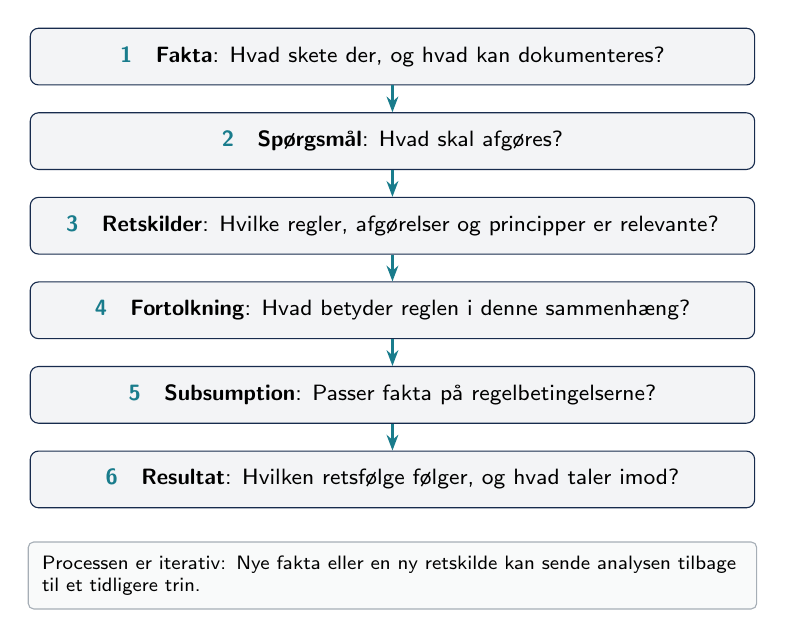
\begin{tikzpicture}[
  node distance=0.34cm,
  block/.style={draw=ink,fill=ink!5,rounded corners=3pt,minimum width=9.2cm,minimum height=.72cm,align=left,inner xsep=.45cm,font=\sffamily\footnotesize},
  arrow/.style={-{Stealth[length=2mm]},thick,accent},
  note/.style={draw=muted!55,fill=softgray!45,rounded corners=2pt,text width=8.9cm,align=left,inner sep=5pt,font=\sffamily\scriptsize}
]
\node[block] (facts) {\textcolor{accent}{\textbf{1}}\quad \textbf{Fakta}: Hvad skete der, og hvad kan dokumenteres?};
\node[block,below=of facts] (question) {\textcolor{accent}{\textbf{2}}\quad \textbf{Spørgsmål}: Hvad skal afgøres?};
\node[block,below=of question] (sources) {\textcolor{accent}{\textbf{3}}\quad \textbf{Retskilder}: Hvilke regler, afgørelser og principper er relevante?};
\node[block,below=of sources] (interpret) {\textcolor{accent}{\textbf{4}}\quad \textbf{Fortolkning}: Hvad betyder reglen i denne sammenhæng?};
\node[block,below=of interpret] (subsume) {\textcolor{accent}{\textbf{5}}\quad \textbf{Subsumption}: Passer fakta på regelbetingelserne?};
\node[block,below=of subsume] (result) {\textcolor{accent}{\textbf{6}}\quad \textbf{Resultat}: Hvilken retsfølge følger, og hvad taler imod?};
\draw[arrow] (facts) -- (question);
\draw[arrow] (question) -- (sources);
\draw[arrow] (sources) -- (interpret);
\draw[arrow] (interpret) -- (subsume);
\draw[arrow] (subsume) -- (result);
\node[note,below=0.42cm of result] {Processen er iterativ: Nye fakta eller en ny retskilde kan sende analysen tilbage til et tidligere trin.};
\end{tikzpicture}

\caption{En praktisk model for juridisk problemløsning. Arbejdsgangen er iterativ: Nye kilder eller fakta kan ændre spørgsmålet.}
\label{fig:method}
\end{figure}

Først fastlægger man \term{fakta}. En sagsfremstilling indeholder ofte både sikre oplysninger, partsforklaringer, antagelser og vurderende ord. ``Han nægtede at samarbejde'' er ikke den samme type oplysning som ``han sendte en e-mail den 3. maj''. Førstnævnte kræver en fortolkning af adfærd; sidstnævnte kan måske dokumenteres direkte.

Dernæst formulerer man det juridiske \term{spørgsmål}. Et godt spørgsmål peger på en retlig standard: ``Har myndigheden overholdt partshøringsreglerne, før den traf afgørelsen?'' er bedre end ``Var kommunen urimelig?''

\section{Retskilder}

Retskilder er de materialer, som bruges til at identificere, begrunde og kontrollere retlige regler. I dansk ret arbejder man typisk med:

\begin{itemize}
  \item Grundloven og andre forfatningsretlige normer,
  \item love vedtaget af Folketinget,
  \item bekendtgørelser og andre administrative forskrifter,
  \item EU-forordninger, direktiver og traktater,
  \item Den Europæiske Menneskerettighedskonvention og anden international ret,
  \item domstolspraksis og administrativ praksis,
  \item lovforarbejder,
  \item sædvane, juridiske principper og almindelige retsgrundsætninger, og
  \item juridisk litteratur som argumentations- og systematiseringskilde.
\end{itemize}

\begin{figure}[ht]
\centering
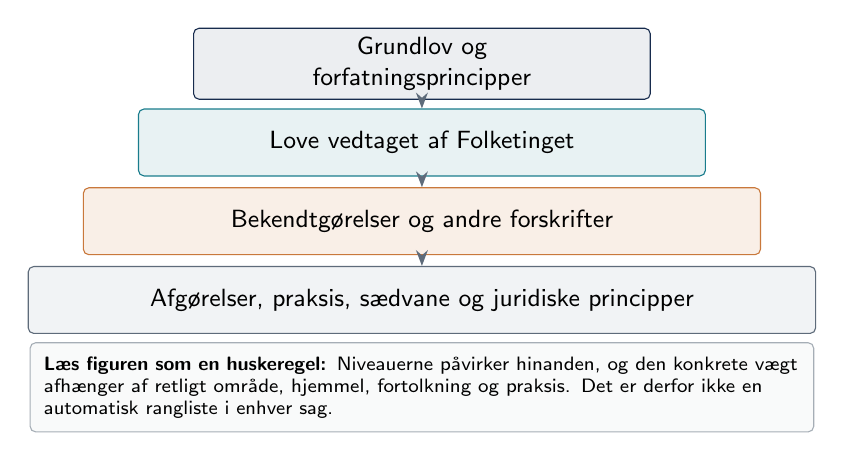
\begin{tikzpicture}[x=1cm,y=0.8cm,
  source/.style={rounded corners=2pt,minimum height=.85cm,align=center,font=\sffamily\small},
  note/.style={draw=muted!55,fill=softgray!45,rounded corners=2pt,text width=9.6cm,align=left,inner sep=5pt,font=\sffamily\scriptsize}
]
  \node[source,draw=ink,fill=ink!8,minimum width=5.8cm] (constitution) at (0,0) {Grundlov og\\forfatningsprincipper};
  \node[source,draw=accent,fill=accent!10,minimum width=7.2cm] (statute) at (0,-1.25) {Love vedtaget af Folketinget};
  \node[source,draw=warm,fill=warm!12,minimum width=8.6cm] (regulation) at (0,-2.5) {Bekendtgørelser og andre forskrifter};
  \node[source,draw=muted,fill=softgray,minimum width=10cm] (practice) at (0,-3.75) {Afgørelser, praksis, sædvane og juridiske principper};
  \draw[-{Stealth[length=2mm]},thick,muted] (constitution.south) -- (statute.north);
  \draw[-{Stealth[length=2mm]},thick,muted] (statute.south) -- (regulation.north);
  \draw[-{Stealth[length=2mm]},thick,muted] (regulation.south) -- (practice.north);
  \node[note,anchor=north] at (0,-4.42) {\textbf{Læs figuren som en huskeregel:} Niveauerne påvirker hinanden, og den konkrete vægt afhænger af retligt område, hjemmel, fortolkning og praksis. Det er derfor ikke en automatisk rangliste i enhver sag.};
\end{tikzpicture}

\caption{En forenklet model over centrale retskildetyper. Den viser ikke en automatisk rangorden i enhver sag.}
\label{fig:pyramid}
\end{figure}

En læser skal være forsigtig med ordet ``rang''. En lov står ikke altid bare ``over'' en dom. En dom kan fortolke loven, afgrænse dens rækkevidde eller anvende en overordnet rettighedsnorm. En bekendtgørelse kan udfylde en lov, men kan ikke uden hjemmel udvide myndighedens kompetence. EU-retten og menneskerettighederne har særlige virkninger, som behandles senere.

\section{Lovtekst og fortolkning}

Fortolkning betyder at fastlægge, hvad en tekst betyder i den relevante retlige sammenhæng. Den begynder ofte med ordlyden, men stopper ikke nødvendigvis der.

\begin{description}[style=nextline,leftmargin=0pt,labelindent=0pt]
  \item[Ordlyd] Hvad siger ordene i deres naturlige og juridiske betydning? Er ``skal'' et krav eller kun en hovedregel?
  \item[Systematik] Hvordan passer bestemmelsen sammen med andre bestemmelser i samme lov og i den samlede retsorden?
  \item[Formål] Hvilket problem skal reglen løse, og hvilke hensyn forsøger den at beskytte?
  \item[Forarbejder] Hvad fremgår af lovforslag, betænkninger og bemærkninger? Forarbejder kan belyse formål, men er ikke det samme som lovtekst.
  \item[Praksis] Hvordan har domstole eller myndigheder anvendt reglen i sammenlignelige tilfælde?
  \item[Konsekvenser] Hvilke resultater følger af fortolkningen, og er de forenelige med proportionalitet, lighed og retssikkerhed?
\end{description}

Fortolkning er ikke det samme som fri kreativitet. En fortolkning skal kunne forsvares i kilderne og være loyal over for den retlige kompetence, der har skabt reglen. Samtidig kan en tekst være åben, og juridisk argumentation kan derfor være rimelig uden at være matematisk entydig.

\section{Analogi, modsætningsslutning og afgrænsning}

Hvis en regel regulerer situation A, kan man spørge, om den bør anvendes analogt på en nært beslægtet situation B. Det kræver en begrundelse for, hvorfor det samme hensyn gør sig gældende. Det er ikke nok, at situationerne ligner hinanden overfladisk.

En \term{modsætningsslutning} går den anden vej: Hvis loven udtrykkeligt regulerer A, kan man argumentere for, at B ikke er omfattet. Det er dog kun overbevisende, hvis lovens struktur viser, at forskellen er bevidst og retligt relevant.

I strafferetten er analogisk udvidelse til skade for den tiltalte stærkt begrænset af legalitetsprincippet. I privat- og forvaltningsretten kan analogier også være problematiske, hvis de skaber nye pligter uden tilstrækkeligt grundlag.

\section{Praksis og præcedens}

En dom er både en afgørelse af en konkret sag og et argument i senere sager. Jo højere instans, jo mere autoritet har afgørelsen normalt. Men præjudikatets styrke afhænger også af, om spørgsmålet var nødvendigt for resultatet, hvor klart retten begrundede det, og hvor sammenlignelige de nye fakta er.

Når du læser en dom, så find mindst fem ting:
\begin{enumerate}
  \item de juridiske spørgsmål,
  \item de faktiske omstændigheder, retten lagde til grund,
  \item parternes vigtigste argumenter,
  \item den regel eller standard, retten anvendte, og
  \item forbindelsen mellem reglen, fakta og resultat.
\end{enumerate}

Det er en fejl kun at læse dommens sidste linje. Resultatet kan være snævert, mens begrundelsen rummer et bredere princip - eller omvendt.

\section{Bevis og usikkerhed}

Juridiske konklusioner bygger på en faktuel præmis. Hvis præmissen er usikker, bliver den juridiske konklusion også usikker. Bevisregler afgør, hvordan usikkerheden håndteres. Hvem har bevisbyrden? Hvilken bevisstyrke kræves? Hvilken forklaring er mest troværdig? Er der objektive dokumenter, tidsstempler, vidner eller tekniske spor?

En juridisk tekst bør markere forskellen mellem:
\begin{itemize}
  \item ``det er dokumenteret, at ...'',
  \item ``det er sandsynligt, at ...'',
  \item ``hvis retten lægger til grund, at ...'', og
  \item ``det kan ikke udelukkes, at ...''.
\end{itemize}

\begin{examplebox}
\textbf{Eksempel: et telefonopkald.} En part siger, at en mundtlig aftale blev indgået mandag. Den anden siger tirsdag. Der findes ingen optagelse, men der er en e-mail onsdag, hvor den første part skriver ``som aftalt''. E-mailen beviser ikke nødvendigvis alle aftalens vilkår, men den kan understøtte, at parterne har haft en fælles forståelse. Den juridiske analyse må angive, hvad beviset faktisk belyser.
\end{examplebox}

\section{Den juridiske argumentationsmodel}

En klar juridisk begrundelse kan skrives sådan:

\begin{methodbox}
\textbf{Regel:} Hvilken bestemmelse eller standard er relevant?\\
\textbf{Betingelser:} Hvilke krav skal være opfyldt?\\
\textbf{Fakta:} Hvilke oplysninger er bevist, og hvilke er omstridte?\\
\textbf{Anvendelse:} Hvordan passer de bevist fakta på betingelserne?\\
\textbf{Modargument:} Hvilken nærliggende indvending kan ændre resultatet?\\
\textbf{Konklusion:} Hvad følger, og hvor sikker er konklusionen?
\end{methodbox}

Denne struktur minder om den klassiske juridiske syllogisme, men den er mere ærlig, fordi den viser, hvor fortolkning og bevisvurdering kommer ind. Den hjælper også med at opdage cirkelslutninger: ``Afgørelsen er lovlig, fordi myndigheden havde lov til at træffe den'' siger ikke noget, hvis hjemlen netop er det omstridte spørgsmål.

\question{Find en regel, du møder i hverdagen. Skriv den som en betinget sætning: ``Hvis ..., så ...''. Hvilke ord er uklare? Hvilke fakta skulle du kende for at anvende reglen?}

\section*{Kapitelopsamling}
\begin{itemize}
  \item Metoden går fra fakta og spørgsmål til kilder, fortolkning, subsumption og konklusion.
  \item En lovtekst skal læses i sammenhæng med systematik, formål, forarbejder og praksis.
  \item Praksis skal læses med blik for både resultat, nødvendige præmisser og faktuel sammenhæng.
  \item Bevisusikkerhed skal fremgå af sproget og ikke skjules bag en sikker konklusion.
  \item En god juridisk tekst viser også det stærkeste modargument.
\end{itemize}


\chapter{Grundloven og den retlige stat}

\chapterlead{Forfatningsretten handler om, hvem der må udøve offentlig magt, hvordan magten skal udøves, og hvilke grænser der beskytter borgeren. Grundloven er derfor både en organisationsplan og en beskyttelse mod vilkårlighed.}

\section{Hvorfor en grundlov?}

En almindelig lov kan normalt ændres af et nyt flertal. En grundlov har en særlig status, fordi den fastlægger de rammer, som lovgiveren selv skal arbejde inden for. Den regulerer blandt andet statens institutioner, lovgivningsproceduren, domstolene og flere grundlæggende frihedsrettigheder \citep{grundloven}.

Den danske Grundlov begynder med, at den gælder for alle dele af Danmarks Rige. Den fastlægger en indskrænket-monarkisk regeringsform og indeholder den klassiske opdeling af magten i en lovgivende, udøvende og dømmende funktion. I praksis betyder det ikke, at funktionerne er hermetisk adskilte. Regeringen forbereder lovforslag, Folketinget kontrollerer regeringen, og domstolene fortolker love. Pointen er, at ingen enkelt aktør skal kunne samle al magt uden kontrol.

\section{Magtens tredeling}

\begin{tabularx}{\textwidth}{@{}>{\RaggedRight\arraybackslash}p{2.6cm}X X@{}}
\toprule
\textbf{Funktion} & \textbf{Hovedopgave} & \textbf{Typisk kontrolspørgsmål} \\
\midrule
Lovgivende & Vedtage generelle regler og fastlægge politiske rammer. & Er loven vedtaget efter den krævede procedure og inden for Grundlovens rammer? \\
Udøvende & Gennemføre lovene og træffe konkrete afgørelser. & Har myndigheden kompetence, fulgt proceduren og anvendt skønnet sagligt? \\
Dømmende & Afgøre konkrete tvister og fortolke retten. & Er domstolen uafhængig, og har parterne fået en fair proces? \\
\bottomrule
\end{tabularx}

Opdelingen skal forstås funktionelt. En minister kan have politisk ansvar for en forvaltning, men den konkrete myndighedsafgørelse skal stadig have hjemmel og følge almindelige forvaltningsretlige krav. Domstolene kan ikke frit overtage Folketingets politiske rolle, men de skal kontrollere, om en lov eller afgørelse holder sig inden for højere regler.

\section{Legalitetsprincippet}

\term{Legalitetsprincippet} betyder i sin kerne, at offentlige indgreb over for borgere kræver et retligt grundlag. En myndighed kan ikke skabe en pligt alene ved at sige, at den synes, pligten er nyttig. Jo mere indgribende handlingen er, jo større krav stilles der typisk til hjemlens klarhed.

Princippet har flere sider:
\begin{itemize}
  \item \textbf{Kompetence:} Myndigheden skal være den rette til at træffe beslutningen.
  \item \textbf{Hjemmel:} Der skal være en regel, som bærer indgrebet.
  \item \textbf{Forudsigelighed:} Borgeren skal i rimeligt omfang kunne forstå, hvad der kræves.
  \item \textbf{Ikke-tilbagevirkning:} I strafferetten må en senere, strengere strafregel som udgangspunkt ikke anvendes på tidligere handlinger. Uden for strafferetten må spørgsmålet vurderes efter den konkrete hjemmel, ikrafttrædelsesregel og eventuelle beskyttelsesprincipper.
  \item \textbf{Kontrol:} Der skal være de kontrolmuligheder, som følger af Grundlov, lov og internationale regler; den konkrete adgang til klage eller domstolsprøvelse varierer.
\end{itemize}

Legalitetsprincippet betyder ikke, at enhver detalje skal stå direkte i en lov. Lovgivning kan delegere nærmere regulering til en minister eller myndighed. Men delegation kræver et tilstrækkeligt grundlag, og den underordnede regel må holde sig inden for rammen.

\section{Delegation og bekendtgørelser}

En lov kan for eksempel sige, at ministeren kan fastsætte nærmere regler om tekniske krav til en bygning. Det kan være praktisk, fordi tekniske standarder ændrer sig hurtigere end en lovgivningsproces. Men en bekendtgørelse kan ikke uden videre indføre en helt ny type straf, skat eller indgreb, hvis loven ikke giver hjemmel til det.

Når du læser en bekendtgørelse, skal du derfor også finde den lovbestemmelse, der bemyndiger udstedelsen. Spørg:

\begin{enumerate}
  \item Hvem har udstedt reglen?
  \item Hvilken lovbestemmelse er hjemlen?
  \item Er reglen udstedt på det rigtige område og inden for bemyndigelsen?
  \item Er der særlige krav til høring, offentliggørelse eller ikrafttræden?
\end{enumerate}

\section{Domstolenes rolle}

Domstolene afgør konkrete retstvister. De kan fortolke loven, anvende grundlovsbestemmelser og prøve, om offentlige beslutninger holder sig inden for loven. Domstolskontrol er normalt konkret: Retten tager stilling til den sag, der er forelagt, og ikke til alle tænkelige anvendelser af reglen.

Domstolene har også en institutionel begrænsning. De må ikke erstatte lovgivers politiske valg med deres egne præferencer. Men hvis et politisk valg overskrider en rettighedsbeskyttelse, en kompetenceregel eller en grundlæggende procesregel, er det netop domstolenes funktion at reagere.

\section{Grundlovens frihedsrettigheder}

Grundloven beskytter blandt andet personlig frihed, boligens ukrænkelighed, ejendomsretten, religionsfrihed, ytringsfrihed, foreningsfrihed og forsamlingsfrihed. Beskyttelsen har forskellig ordlyd og forskellig struktur. Nogle bestemmelser kræver lovhjemmel, andre indeholder særlige betingelser, og nogle skal læses sammen med menneskerettighederne.

En grundrettighed er derfor ikke altid et absolut forbud. Mange rettigheder kan begrænses, hvis betingelserne er opfyldt. Det centrale er at identificere:
\begin{itemize}
  \item hvilket beskyttet gode der berøres,
  \item om der faktisk er tale om et indgreb,
  \item om indgrebet har hjemmel,
  \item om det forfølger et legitimt formål, og
  \item om det er proportionalt og underlagt kontrol.
\end{itemize}

\section{Krise, hast og nød}

Krisebestemmelser og nødret rejser et grundlæggende spørgsmål: Kan staten handle hurtigere, når almindelige procedurer er utilstrækkelige? Svaret er ikke, at regler forsvinder, når situationen bliver vanskelig. Tværtimod bliver hjemmel, tidsbegrænsning, nødvendighed, parlamentarisk kontrol og domstolsprøvelse endnu vigtigere.

Nødret er ikke en generel tilladelse til at gøre, hvad der føles rigtigt. Den kræver en konkret vurdering af fare, nødvendighed, proportionalitet og alternativer. Hvad der var nødvendigt under en akut fare, er ikke nødvendigvis nødvendigt, når faren er aftaget.

\question{En kommune vil af sikkerhedshensyn lukke en offentlig plads efter flere urolige aftener. Hvilke spørgsmål om kompetence, hjemmel, proportionalitet, varighed og kontrol skal stilles, før du vurderer, om beslutningen er lovlig?}

\section*{Kapitelopsamling}
\begin{itemize}
  \item Grundloven fordeler magt og beskytter grundlæggende interesser.
  \item Magtens tredeling er en arbejdsdeling med gensidig kontrol, ikke tre isolerede verdener.
  \item Offentlige indgreb kræver kompetence, hjemmel, forudsigelighed og kontrol.
  \item Delegation er mulig, men en bekendtgørelse må holde sig inden for lovens ramme.
  \item Grundrettigheder kan ofte begrænses, men kun efter krav om blandt andet hjemmel og proportionalitet.
\end{itemize}

\chapter{Offentlig forvaltning og god sagsbehandling}

\chapterlead{Forvaltningsret er den del af retten, der omsætter offentlig magt til konkrete afgørelser. Den beskytter borgeren gennem krav til kompetence, oplysning, upartiskhed, høring, begrundelse og klage.}

\section{Fra lov til afgørelse}

En lov er ofte generel. Den siger eksempelvis, at personer, der opfylder bestemte betingelser, kan få en ydelse, eller at en virksomhed skal have en tilladelse. Forvaltningen skal anvende reglen på en konkret person, virksomhed eller situation. Det kræver både faktumindsamling og juridisk vurdering.

Forvaltningsloven gælder som hovedregel for behandlingen af sager, hvor en forvaltningsmyndighed træffer eller skal træffe en afgørelse, og indeholder også regler om blandt andet inhabilitet, partsaktindsigt, partshøring, begrundelse og klagevejledning \citep{forvaltningsloven}. Offentlighedsloven regulerer en bredere adgang til aktindsigt i den offentlige forvaltning \citep{offentlighedsloven}.

\section{Kompetence}

Før man spørger, om en afgørelse er rimelig, må man spørge, om den rette myndighed har truffet den. Kompetence kan være:
\begin{itemize}
  \item \textbf{Saglig:} Hvilken type spørgsmål må myndigheden tage stilling til?
  \item \textbf{Stedlig:} Hvilket geografisk område eller hvilken kommune er relevant?
  \item \textbf{Personel:} Hvem i organisationen må træffe afgørelsen?
  \item \textbf{Tidsmæssig:} Gælder kompetencen på det tidspunkt, hvor beslutningen blev truffet?
\end{itemize}

En myndighed kan godt have kompetence til at behandle en sag, men ikke til at træffe alle tænkelige beslutninger i den. Det er også nødvendigt at undersøge, om afgørelsen er truffet af den rette person eller efter de krav om delegation, som gælder internt og eksternt.

\section{Inhabilitet og upartiskhed}

En sagsbehandler er inhabil, hvis der foreligger forhold, som kan rejse tvivl om vedkommendes upartiskhed. Det kan være en personlig eller økonomisk interesse, et nært forhold til en part eller tidligere medvirken på en måde, der gør den nye behandling problematisk.

Reglen beskytter ikke kun mod faktisk partiskhed. Den beskytter også tilliden til afgørelsen. Derfor er spørgsmålet ikke altid, om personen faktisk lod sig påvirke, men om situationen udefra giver en rimelig grund til tvivl.

\section{Oplysningsgrundlag og officialprincippet}

Den offentlige myndighed har som udgangspunkt ansvar for, at sagen er tilstrækkeligt oplyst, før den træffer afgørelse. Dette kaldes ofte officialprincippet. Omfanget afhænger af sagstype, indgrebets styrke, oplysningernes tilgængelighed og parternes mulighed for selv at fremskaffe dem.

Et tilstrækkeligt oplysningsgrundlag betyder ikke, at alle tænkelige oplysninger skal indsamles. Det betyder, at myndigheden må kende de fakta, der er nødvendige for at anvende den relevante regel forsvarligt. Et alvorligt indgreb kræver typisk større omhu end en rutinemæssig servicebeslutning.

\begin{examplebox}
\textbf{Eksempel: støtte og indtægt.} Hvis en myndighed skal afgøre, om en borger opfylder et indtægtskrav, må den undersøge den relevante periode, den relevante indkomsttype og eventuelle undtagelser. Det er ikke nok at se på ét tilfældigt kontoudtog, hvis reglen kræver en samlet opgørelse. Omvendt er myndigheden heller ikke forpligtet til at undersøge forhold, der åbenlyst ikke kan påvirke resultatet.
\end{examplebox}

\section{Partshøring}

Partshøring giver parten mulighed for at kommentere væsentlige faktiske oplysninger, som myndigheden vil bruge til ugunst for parten, og som parten ikke kan antages at kende, med de undtagelser der følger af loven. Høringen skal være reel: Parten skal have en rimelig mulighed for at forstå oplysningerne og svare, før afgørelsen træffes.

Høringspligten er ikke det samme som en ret til at bestemme resultatet. Den er en ret til at blive hørt og til at kunne korrigere fejl, forklare kontekst eller fremlægge nye oplysninger. Manglende høring kan få betydning for afgørelsens gyldighed, men virkningen afhænger af den konkrete sag og af, om fejlen kan have haft betydning.

\section{Begrundelse og klagevejledning}

En begrundelse gør afgørelsen forståelig og kontrollerbar. Den bør vise:
\begin{enumerate}
  \item hvilket retsgrundlag myndigheden har brugt,
  \item hvilke hovedhensyn der har været bestemmende ved et skøn, og
  \item hvilke faktiske oplysninger myndigheden har lagt til grund.
\end{enumerate}

En begrundelse er mere end en konklusion. ``Du opfylder ikke betingelserne'' giver sjældent parten mulighed for at vurdere, om myndigheden har forstået sagen rigtigt. En kort afgørelse kan være lovlig, hvis sagen er enkel, men enkelhed skal ikke bruges som undskyldning for at skjule det afgørende ræsonnement.

Når en afgørelse kan påklages, skal klagevejledningen normalt fortælle, til hvem og inden for hvilken frist. Ikke alle afgørelser har en administrativ klageadgang, og den konkrete regel skal derfor kontrolleres. En uklar eller manglende vejledning kan påvirke partens muligheder for at reagere, men den konkrete virkning afhænger af reglerne og omstændighederne.

\section{Skøn, lighed og saglighed}

En regel kan give myndigheden et skøn. Skøn betyder ikke, at myndigheden må vælge helt frit. Skønnet skal holdes inden for lovens formål, bygge på relevante hensyn og respektere lighed og proportionalitet.

\begin{description}[style=nextline,leftmargin=0pt,labelindent=0pt]
  \item[Saglighed] Hensynene skal have forbindelse til den opgave, loven regulerer. Personlige sympatier eller irrelevante politiske ønsker må ikke styre afgørelsen.
  \item[Lighed] Væsentligt ens sager skal behandles ens, medmindre der er en relevant forskel.
  \item[Proportionalitet] Indgrebet skal være egnet, nødvendigt og rimeligt i forhold til formålet.
  \item[Magtfordrejning og skønsgrænser] En myndighed må ikke lade irrelevante hensyn styre eller gøre en hovedregel til en absolut regel, hvis loven forudsætter individuel vurdering.
  \item[Berettigede forventninger] En myndigheds tidligere udmeldinger og praksis kan i visse tilfælde begrænse pludselige ændringer, men forventninger kan ikke uden videre fastholde en ulovlig praksis.
\end{description}

\section{Aktindsigt og tavshed}

Aktindsigt gør det muligt at se, hvad en myndighed ved og har lagt vægt på. Retten er ikke ubegrænset. Hensyn til private forhold, sikkerhed, interne arbejdsdokumenter og andre beskyttede interesser kan begrunde undtagelser. Undtagelser skal fortolkes i lyset af lovens formål, og der kan være pligt til meroffentlighed.

Tavshedspligt beskytter oplysninger, som myndigheden ikke må videregive. Aktindsigt og tavshedspligt skal derfor afvejes i hver enkelt sag. At en oplysning findes hos en myndighed, betyder ikke automatisk, at alle har adgang til den.

\section{Kontrol med forvaltningen}

En afgørelse kan kontrolleres af en intern genvurdering, en administrativ klageinstans, Folketingets Ombudsmand, domstolene eller et særligt nævn. Kontrollen kan være retlig, faglig eller begge dele. En klageinstans kan nogle gange prøve hele sagen, mens domstolen typisk fokuserer på retlige spørgsmål og grænserne for forvaltningens skøn.

\practice{Når du vurderer en myndighedsafgørelse, skriv først en tidslinje. Marker derefter: kompetence, faktagrundlag, høring, hjemmel, skøn, begrundelse, klagevejledning og tidsfrister. Først derefter vurderer du, om resultatet virker rimeligt.}

\question{En myndighed ændrer en borgers ydelse med virkning fra næste måned. Afgørelsen nævner kun et nyt internt notat og skriver, at ``reglerne er blevet strammet''. Hvilke oplysninger og juridiske spørgsmål mangler du?}

\section*{Kapitelopsamling}
\begin{itemize}
  \item En myndighed skal have kompetence og et tilstrækkeligt hjemmelsgrundlag.
  \item Sagen skal være tilstrækkeligt oplyst, og parten skal høres, når reglerne kræver det.
  \item Begrundelsen skal gøre retsgrundlag, faktum og afgørende hensyn kontrollerbare.
  \item Skøn er bundet af saglighed, lighed, proportionalitet og lovens formål.
  \item Aktindsigt, klage og domstolskontrol er centrale retssikkerhedsmekanismer.
\end{itemize}

\chapter{Grundlæggende rettigheder og proportionalitet}

\chapterlead{Rettigheder beskytter mennesker mod visse indgreb og giver dem krav på bestemte former for respekt, procedure og lighed. Rettighedsanalyse kræver, at man identificerer både beskyttelsen, indgrebet, hjemlen og afvejningen.}

\section{Hvad er en rettighed?}

En rettighed kan være et krav på, at andre gør noget, en frihed til at handle uden indgreb, en kompetence til at ændre en retlig situation eller en immunitet mod en bestemt type beslutning. Når man siger ``ytringsfrihed'', mener man ikke kun retten til at tale. Man mener også regler om, hvornår staten må straffe, censurere eller pålægge ansvar for en ytring.

Rettigheder har ofte flere dimensioner:
\begin{itemize}
  \item en \textbf{negativ} dimension: staten skal afstå fra indgreb,
  \item en \textbf{positiv} dimension: staten skal i visse situationer beskytte eller tilvejebringe noget, og
  \item en \textbf{procedurel} dimension: personen skal have adgang til information, høring, klage eller domstolsprøvelse.
\end{itemize}

\section{Flere beskyttelseslag}

I Danmark kan en rettighed være beskyttet af Grundloven, Den Europæiske Menneskerettighedskonvention, EU-rettens charter og almindelig lovgivning. Lagene overlapper, men de er ikke ens. De har forskellige ordlyder, institutioner, fortolkningspraksisser og retsvirkninger.

ECHR-systemet, det vil sige konventionen sammen med tillægsprotokollerne, beskytter blandt andet retten til liv, forbud mod tortur, personlig frihed, retfærdig rettergang, privatliv, religionsfrihed, ytringsfrihed og ejendomsbeskyttelse \citep{echr}. EU-charteret indeholder blandt andet bestemmelser om privatliv, persondata, ytringsfrihed og effektiv domstolsbeskyttelse \citep{charter}. Charteret gælder, når medlemsstaterne handler inden for EU-rettens anvendelsesområde.

\section{Er der et indgreb?}

Før man diskuterer, om et indgreb er rimeligt, skal man identificere, hvad der faktisk er sket. Et indgreb kan være direkte, som et forbud eller en frihedsberøvelse. Det kan også være indirekte, som en sanktion, der gør det meget vanskeligt at udøve en rettighed.

Det er vigtigt ikke at definere indgrebet så snævert, at problemet forsvinder. Omvendt skal enhver praktisk ulempe heller ikke behandles som et rettighedsindgreb. Man må vurdere regelens formål, virkning, intensitet og forbindelse til den beskyttede interesse.

\section{Proportionalitet}

Proportionalitet er en måde at teste, om et indgreb går længere end nødvendigt. Den kan udtrykkes i fem spørgsmål:

\begin{figure}[ht]
\centering
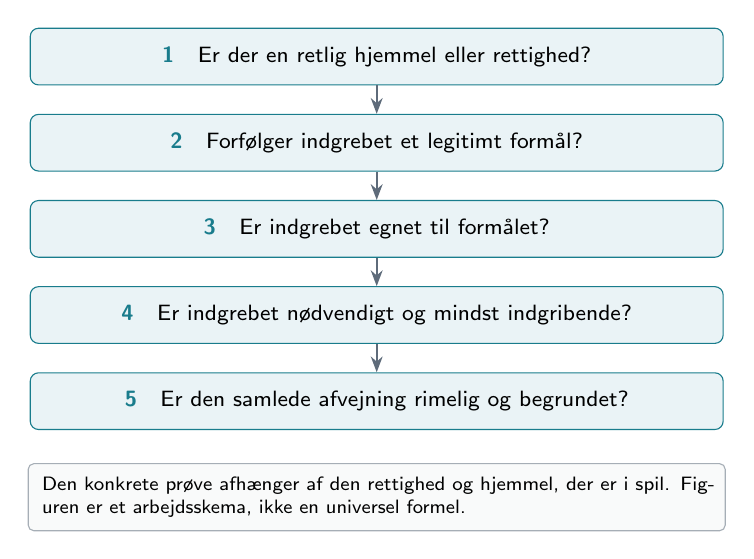
\begin{tikzpicture}[
  node distance=0.36cm,
  test/.style={draw=accent,fill=softblue,rounded corners=3pt,minimum width=8.8cm,minimum height=.72cm,align=left,inner xsep=.42cm,font=\sffamily\footnotesize},
  arrow/.style={-{Stealth[length=2mm]},thick,muted},
  note/.style={draw=muted!55,fill=softgray!45,rounded corners=2pt,text width=8.5cm,align=left,inner sep=5pt,font=\sffamily\scriptsize}
]
\node[test] (basis) {\textcolor{accent}{\textbf{1}}\quad Er der en retlig hjemmel eller rettighed?};
\node[test,below=of basis] (purpose) {\textcolor{accent}{\textbf{2}}\quad Forfølger indgrebet et legitimt formål?};
\node[test,below=of purpose] (suitable) {\textcolor{accent}{\textbf{3}}\quad Er indgrebet egnet til formålet?};
\node[test,below=of suitable] (necessary) {\textcolor{accent}{\textbf{4}}\quad Er indgrebet nødvendigt og mindst indgribende?};
\node[test,below=of necessary] (balance) {\textcolor{accent}{\textbf{5}}\quad Er den samlede afvejning rimelig og begrundet?};
\draw[arrow] (basis) -- (purpose);
\draw[arrow] (purpose) -- (suitable);
\draw[arrow] (suitable) -- (necessary);
\draw[arrow] (necessary) -- (balance);
\node[note,below=0.42cm of balance] {Den konkrete prøve afhænger af den rettighed og hjemmel, der er i spil. Figuren er et arbejdsskema, ikke en universel formel.};
\end{tikzpicture}

\caption{En praktisk proportionalitetsprøvelse. Den præcise test afhænger af den relevante bestemmelse.}
\label{fig:rights-test}
\end{figure}

Et indgreb kan være egnet, men stadig unødvendigt, hvis et mindre indgribende middel kunne nå samme formål. Et indgreb kan også være nødvendigt, men samlet set for byrdefuldt for den enkelte. Proportionalitet er derfor ikke kun et spørgsmål om effektivitet; det er også en afvejning af rettighedens vægt og indgrebets intensitet.

\begin{examplebox}
\textbf{Eksempel: adgangskontrol.} En offentlig institution indfører krav om identifikation ved indgangen for at beskytte sikkerheden. Spørgsmålet er ikke alene, om sikkerhed er et legitimt formål. Man må også spørge, hvilke oplysninger der indsamles, hvor længe de gemmes, om alle skal registreres, om anonyme alternativer findes, og om kontrollen kan målrettes mindre indgribende.
\end{examplebox}

\section{Ytrings- og informationsfrihed}

Ytringsfrihed beskytter både politiske udtalelser, kunstneriske udtryk, journalistik og mange former for hverdagskommunikation. Beskyttelsen kan variere efter ytringens karakter og indgrebets form. Politisk tale har normalt en stærk beskyttelse, mens trusler, injurier eller ulovlige opfordringer kan være reguleret.

Juridisk analyse bør skelne mellem:
\begin{itemize}
  \item indholdet i ytringen,
  \item formen og mediet,
  \item hvem der regulerer ytringen,
  \item sanktionens størrelse og karakter, og
  \item det formål, som begrænsningen skal varetage.
\end{itemize}

At en ytring er stødende eller falsk, er ikke altid nok til at gøre den ulovlig. At en ytring er politisk, gør den heller ikke automatisk lovlig. Den juridiske vurdering kræver den konkrete bestemmelse og de relevante beskyttelseshensyn.

\section{Privatliv, hjem og data}

Privatliv beskytter ikke kun hemmeligheder. Det omfatter også personlig identitet, relationer, kommunikation, hjem og kontrol over personlige oplysninger. Digitale teknologier gør spørgsmålet mere komplekst, fordi en enkelt oplysning kan virke harmløs, mens kombinationen af mange oplysninger kan afsløre helbred, vaner, økonomi og politiske holdninger.

En stat kan have legitime grunde til overvågning, registrering eller kontrol. Men jo mere systematisk og omfattende indgrebet er, desto større krav stilles der typisk til klar hjemmel, nødvendighed, adgangsbegrænsning, sletning, tilsyn og effektive klagemuligheder.

\section{Ejendom og økonomisk frihed}

Ejendomsbeskyttelse betyder ikke, at ejeren aldrig kan reguleres. Samfundet kan fastsætte planregler, skatter, miljøkrav og sikkerhedskrav. Spørgsmålet er, om reguleringen blot er en almindelig begrænsning af brugen, eller om der reelt sker en ekspropriation eller et andet intensivt indgreb. Her er formål, varighed, økonomisk virkning og muligheden for fortsat anvendelse centrale.

\section{Retfærdig rettergang}

Retten til en fair proces handler blandt andet om adgang til en domstol, uafhængighed og upartiskhed, rimelig sagsbehandlingstid, kontradiktion, lighed mellem parterne og mulighed for at få prøvet afgørelsen. En retfærdig rettergang er ikke nødvendigvis en proces, hvor man får det resultat, man ønsker. Det er en proces, hvor resultatet er fremkommet gennem regler, der beskytter parternes mulighed for at deltage og blive hørt.

\section{Lighed og diskrimination}

Lighed betyder ikke altid identisk behandling. En forskelsbehandling kan være relevant, hvis personer er i forskellige situationer, eller hvis et legitimt formål kræver en målrettet forskel. Omvendt kan en tilsyneladende neutral regel ramme en bestemt gruppe skævt. Derfor må man undersøge både regelens ordlyd, praksis og virkning.

\caution{Rettighedsargumenter skal være præcise. Skriv ikke blot ``det krænker mine rettigheder''. Angiv den konkrete rettighed, indgrebet, hjemlen, formålet, proportionalitetsproblemet og den prøvelsesmulighed, du påberåber dig.}

\question{En uddannelsesinstitution vil bruge ansigtsgenkendelse ved eksamensindgange for at forhindre snyd. Hvilke rettigheder og proportionalitetsspørgsmål opstår, før man overhovedet vurderer, om teknologien virker?}

\section*{Kapitelopsamling}
\begin{itemize}
  \item Rettigheder kan være krav, friheder, kompetencer og processuelle garantier.
  \item Grundloven, ECHR, EU-charteret og almindelig lov kan beskytte samme interesse på forskellige måder.
  \item Rettighedsanalyse kræver en konkret identifikation af indgrebet og hjemlen.
  \item Proportionalitet spørger til formål, egnethed, nødvendighed og samlet rimelighed.
  \item Lighed kræver analyse af både forskelsbehandlingens grund og dens faktiske virkning.
\end{itemize}

\chapter{EU-ret og international ret}

\chapterlead{Dansk ret eksisterer i et lagdelt retssystem. EU-retten kan have direkte betydning i Danmark, mens internationale konventioner får virkning gennem traktat, lovgivning og fortolkning. Den juridiske opgave er at finde det rigtige lag og forstå forbindelsen mellem dem.}

\section{Hvorfor er EU-ret relevant?}

EU-retten regulerer områder som det indre marked, forbrugerbeskyttelse, databeskyttelse, konkurrence, miljø, migration og digital regulering. En dansk sag kan derfor være underlagt både en dansk lov og en EU-forordning eller et direktiv.

EU-rettens vigtigste retskilder er traktaterne, forordninger, direktiver, afgørelser, Domstolen for Den Europæiske Unions praksis og visse generelle principper. EU-charteret beskytter grundlæggende rettigheder, når medlemsstaterne gennemfører eller anvender EU-ret.

\section{Forordninger og direktiver}

En EU-forordning gælder som udgangspunkt direkte i medlemsstaterne. Den skal ikke først omskrives til en dansk lov for at have virkning, selv om national lovgivning kan være nødvendig for at organisere myndigheder, sanktioner og procedurer.

Et direktiv fastlægger et resultat, som medlemsstaterne skal nå, men overlader ofte valg af form og midler til national gennemførelse. Man skal derfor finde både direktivet og den danske gennemførelseslov, når man arbejder med en direktivbaseret regel.

\begin{tabularx}{\textwidth}{@{}>{\RaggedRight\arraybackslash}p{2.7cm}X X@{}}
\toprule
\textbf{Instrument} & \textbf{Grundidé} & \textbf{Spørgsmål i en konkret sag} \\
\midrule
Forordning & Ensartede regler, der som udgangspunkt gælder direkte. & Hvilke bestemmelser og overgangsregler gælder, og hvilken national myndighed håndhæver dem? \\
Direktiv & Bindende mål, der normalt kræver national gennemførelse. & Hvilken dansk regel gennemfører direktivet, og skal den fortolkes direktivkonformt? \\
Traktat & EU's overordnede kompetencer, institutioner og principper. & Er området omfattet af EU's kompetence, og hvilken traktatbestemmelse er relevant? \\
Domstols-\\praksis & Fortolker og konkretiserer EU-retten. & Hvilken retlig test og hvilke betingelser har EU-Domstolen fastlagt? \\
\bottomrule
\end{tabularx}

\section{Forrang og effektivitet}

EU-rettens forrang betyder i hovedtræk, at modstridende national ret må vige inden for EU-rettens anvendelsesområde. Forrang er ikke det samme som, at EU kan regulere alle emner. Først skal man finde en gyldig EU-kompetence og den relevante EU-regel.

National ret skal så vidt muligt fortolkes i overensstemmelse med EU-retten. Hvis en konflikt ikke kan løses gennem fortolkning, kan den nationale domstol skulle undlade at anvende den modstridende nationale regel i den konkrete sag. Den præcise virkning afhænger af regeltype, parternes relation og EU-rettens betingelser.

\section{Præjudicielle spørgsmål}

Hvis en dansk domstol er i tvivl om fortolkningen eller gyldigheden af EU-retten, kan den forelægge spørgsmålet for EU-Domstolen. En forelæggelse er ikke en almindelig appel. Den nationale ret beholder ansvaret for at afgøre den konkrete sag, efter at EU-Domstolen har besvaret det EU-retlige spørgsmål.

Metodisk er pointen: Hvis resultatet afhænger af et uklart EU-retligt begreb, skal man søge EU-Domstolens praksis og ikke kun læse den danske lov.

\section{International ret og dansk ret}

Internationale traktater binder Danmark på folkeretligt plan. Den nationale virkning afhænger af, hvordan traktaten er gennemført eller indarbejdet i dansk ret. Nogle konventioner får betydning gennem en dansk gennemførelseslov; andre påvirker fortolkningen af national ret eller statens internationale ansvar.

Den Europæiske Menneskerettighedskonvention er inkorporeret i dansk ret og har stor betydning for domstole og myndigheder \citep{echr,menneskerettighedsloven}. Den Europæiske Menneskerettighedsdomstols praksis bruges til at forstå konventionens dynamiske anvendelse, men enhver sag kræver opmærksomhed på den konkrete artikel, den konkrete indgrebsform og statens skønsmargin.

\section{Et EU-retligt arbejdsskema}

\practice{Når en sag kan have EU-retlige elementer, så spørg: (1) Er faktum inden for et EU-reguleret område? (2) Hvilken traktatbestemmelse eller EU-retsakt er relevant? (3) Er det en forordning, et direktiv eller en anden retskilde? (4) Findes der dansk gennemførelseslov? (5) Hvad siger EU-Domstolens praksis? (6) Er Charteret relevant? (7) Er der en konflikt med national ret?}

\section{Eksempel: persondata}

En dansk virksomhed bruger en amerikansk cloudtjeneste til at behandle kundedata. Spørgsmålet er ikke kun, om virksomheden følger dansk databeskyttelseslov. Man må også anvende GDPR, vurdere rollerne som dataansvarlig og databehandler, undersøge overførsel til tredjelande og se på eventuelle supplerende danske regler. Hvis teknologien bruger kunstig intelligens, kan AI-forordningen give yderligere pligter, afhængigt af systemets anvendelse, aktørens rolle og den relevante anvendelsesdato.

\section{EU-rettens begrænsninger}

Det er en fejl at bruge EU-retten som et generelt argument for alt. EU har kun de kompetencer, som medlemsstaterne har overladt gennem traktaterne. En sag uden tilstrækkelig forbindelse til EU-rettens område kan ikke automatisk bringes ind under Charteret eller EU's regler.

Det er også en fejl at antage, at alle EU-regler er ensartede. Medlemsstaterne kan have forskellige institutioner, sanktioner og procedurer, så længe de overholder EU-rettens krav om blandt andet effektivitet, ækvivalens og loyal gennemførelse.

\question{En dansk kommune bruger en EU-forordning som begrundelse for et indgreb, men kan ikke pege på den konkrete artikel. Hvad skal du undersøge, før du accepterer henvisningen?}

\section*{Kapitelopsamling}
\begin{itemize}
  \item EU-retten er et integreret lag i mange danske retsområder.
  \item Forordninger gælder som udgangspunkt direkte; direktiver kræver normalt national gennemførelse.
  \item EU-rettens forrang gælder inden for EU-rettens anvendelsesområde.
  \item Internationale konventioners nationale virkning afhænger af traktatens status og dansk gennemførelse.
  \item Begynd altid med kompetence og den konkrete retskilde, ikke med en abstrakt henvisning til ``EU''.
\end{itemize}

\chapter{Aftaler, forbrugerkøb og misligholdelse}

\chapterlead{Aftaler gør løfter retligt forpligtende. Aftaleretten spørger, om der er indgået en aftale, hvad den betyder, om den er gyldig, og hvad der sker, hvis en part ikke leverer som aftalt.}

\section{Fra samtale til bindende aftale}

Mennesker laver aftaler hele tiden: køb af kaffe, leje af bolig, abonnement på software, ansættelse og lån af penge. Ikke alle sociale løfter er juridisk bindende. Juraen må skelne mellem en venlig hensigt, en invitation til at forhandle og en aftale, der kan håndhæves.

Klassisk aftaleret beskriver processen som tilbud og accept. Et tilbud er tilstrækkeligt bestemt og viser en vilje til at blive bundet, hvis modtageren accepterer inden for fristen. En accept skal normalt stemme med tilbuddet. En ændret accept kan være et nyt tilbud, selv om parterne i praksis ofte udveksler flere beskeder, før det står klart, hvad de er enige om.

Aftaleloven indeholder centrale regler om tilbud, accept, fuldmagt og ugyldighed \citep{aftaleloven}. Men aftaleretten består også af almindelige principper, branchepraksis, forbrugerregler og den konkrete aftales ordlyd.

\section{Aftalens indhold}

Når parterne er enige om hovedydelsen, kan der stadig være tvivl om pris, levering, kvalitet, opsigelse, ansvar og ændringer. Aftalens indhold findes gennem en samlet fortolkning:

\begin{itemize}
  \item Hvad står der i kontrakten?
  \item Hvilke oplysninger blev givet før aftalen?
  \item Hvilken betydning har parternes efterfølgende adfærd?
  \item Hvilken branche eller type aftale er der tale om?
  \item Er et vilkår uklart, overraskende eller urimeligt?
  \item Gælder præceptive regler, som parterne ikke kan fravige?
\end{itemize}

En kontrakt er ikke kun den lange tekst, som parterne underskriver. Tilbud, ordrebekræftelse, standardvilkår, bilag, e-mails og mundtlige udsagn kan tilsammen udgøre aftalegrundlaget. Derfor skal man bevare hele forløbet, ikke kun den sidste PDF.

\section{Fuldmagt}

En person kan handle på en andens vegne. Hvis den, der handler, har fuldmagt, kan handlingen binde den repræsenterede over for tredjemand. Det afgørende kan være forskellen mellem den interne bemyndigelse og den ydre legitimation:

\begin{description}[style=nextline,leftmargin=0pt,labelindent=0pt]
  \item[Intern bemyndigelse] Hvad har hovedpersonen faktisk sagt til fuldmægtigen, at denne må gøre?
  \item[Legitimation] Hvad har tredjemand rimelig grund til at tro, at fuldmægtigen må gøre?
  \item[Overskridelse] Hvad sker der, hvis fuldmægtigen går længere end den interne besked?
\end{description}

Fuldmagtsproblemer opstår ofte i virksomheder, hvor en medarbejder har en titel eller funktion, der normalt giver omverdenen en bestemt forventning. Vurderingen afhænger af fuldmagtens art og tredjemands gode eller onde tro.

\section{Ugyldighed}

En aftale kan være ugyldig, hvis den er fremkaldt ved tvang, svig eller udnyttelse, hvis erklæringen er afgivet ved en fejl, eller hvis aftalen strider mod ufravigelige regler. Ugyldighed er ikke en samlet etikette; forskellige ugyldighedsgrunde har forskellige betingelser og retsvirkninger.

Man skal blandt andet spørge:
\begin{itemize}
  \item Hvilken ugyldighedsgrund påberåbes?
  \item Hvem kendte eller burde kende det forhold, der gør aftalen problematisk?
  \item Har den berørte reageret hurtigt nok?
  \item Har tredjemand indrettet sig i tillid til aftalen?
  \item Er hele aftalen ugyldig, eller kun et bestemt vilkår?
\end{itemize}

\section{Misligholdelse}

Misligholdelse betyder, at en part ikke opfylder aftalen korrekt. Det kan være forsinkelse, mangler, manglende betaling eller en anden afvigelse fra det aftalte.

\begin{tabularx}{\textwidth}{@{}>{\RaggedRight\arraybackslash}p{2.4cm}X X@{}}
\toprule
\textbf{Retsfølge} & \textbf{Hvad betyder det?} & \textbf{Typisk spørgsmål} \\
\midrule
Opfyldelse & Den anden part kræver den aftalte ydelse. & Kan ydelsen stadig leveres, og er kravet begrænset af regler eller umulighed? \\
Afhjælpning & Fejlen rettes, eller varen omleveres. & Er det praktisk muligt, rimeligt og rettidigt? \\
Prisafslag & Prisen reduceres, fordi ydelsen er mindre værd. & Hvor stor er værdiforringelsen? \\
Ophævelse & Aftalen bringes til ophør på grund af væsentlig misligholdelse. & Er misligholdelsen væsentlig, og er der reklameret rettidigt? \\
Erstatning & Tab erstattes efter de relevante betingelser. & Er der ansvar, tab og årsagssammenhæng? \\
\bottomrule
\end{tabularx}

Den rigtige reaktion afhænger af aftalen og den relevante lov. Man kan ikke automatisk ophæve, fordi noget er irriterende, eller kræve erstatning, fordi man er skuffet. Væsentlighed, reklamation, tabsbegrænsning og forudsigelighed kan være afgørende.

\section{Forbrugerkøb}

Når en forbruger køber en vare af en erhvervsdrivende, gælder særlige beskyttelsesregler. Købeloven indeholder blandt andet regler om mangler, levering, reklamation og beføjelser. Den har også regler om varer med digitale elementer; digitalt indhold og digitale tjenester kan desuden være reguleret af særregler i forbrugerretten. Hvilket regelsæt der gælder, afhænger af ydelsens type og parternes status \citep{koebeloven}.

Forbrugeren kan normalt ikke stilles dårligere end den beskyttelse, som ufravigelige regler giver. Det betyder ikke, at forbrugeren altid vinder en tvist. Man skal stadig dokumentere købet, beskrive manglen, reklamere inden for reglernes rammer og give sælgeren mulighed for at afhjælpe, når det kræves.

\section{Digitale ydelser}

Et abonnement på en streamingtjeneste eller en cloudplatform er ikke identisk med køb af en fysisk ting. Ydelsen kan bestå af adgang, løbende opdateringer, behandling af persondata og en licens til software. Det gør det vigtigt at identificere, hvad leverandøren faktisk har lovet, og hvilke regler der gælder for ændringer, afbrydelser og data.

\begin{examplebox}
\textbf{Eksempel: den ændrede tjeneste.} En bruger betaler for en app med en bestemt funktion. Leverandøren fjerner funktionen og henviser til standardvilkårene, som siger, at tjenesten kan ændres. Vurderingen kræver, at man læser vilkårets ordlyd, ændringens betydning, informationen til brugeren, eventuelle forbrugerregler og spørgsmålet om, hvorvidt den aftalte hovedydelse reelt er ændret.
\end{examplebox}

\section{Kontraktlæsning i praksis}

Læs aldrig en kontrakt som en liste af enkeltord. Find først aftalens struktur:
\begin{enumerate}
  \item Hvem er parterne, og hvilken kapacitet handler de i?
  \item Hvad er hovedydelserne?
  \item Hvornår og hvordan skal der leveres?
  \item Hvilke risici og undtagelser reguleres?
  \item Hvordan kan aftalen ændres eller opsiges?
  \item Hvilken lov og hvilken tvistløsningsmekanisme gælder?
  \item Er et standardvilkår uklart, overraskende eller urimeligt?
\end{enumerate}

\caution{Et vilkår med overskriften ``ansvarsfraskrivelse'' er ikke nødvendigvis gyldigt eller dækkende. Spørg altid, hvilken skade, hvilken adfærd og hvilken part vilkåret faktisk omfatter.}

\question{Du bestiller en speciallavet reol. Den leveres tre uger for sent og passer ikke til den oplyste niche. Hvilke forskellige krav kan være relevante, og hvilke fakta afgør, om du kan hæve aftalen?}

\section*{Kapitelopsamling}
\begin{itemize}
  \item En aftale kræver en retligt relevant overensstemmelse, ikke blot en social forventning.
  \item Aftalens indhold findes i ordlyd, forløb, praksis, branche og præceptive regler.
  \item Fuldmagt handler både om intern bemyndigelse og tredjemands legitime forventning.
  \item Misligholdelse kan udløse forskellige beføjelser, som kræver forskellige betingelser.
  \item Forbrugerkøb og digitale ydelser er præget af ufravigelig beskyttelse og EU-regler.
\end{itemize}

\chapter{Erstatning og ansvar}

\chapterlead{Erstatningsretten fordeler risikoen for et tab. Den spørger, om nogen har handlet ansvarspådragende, om handlingen forårsagede skaden, hvilket tab der kan opgøres, og om andre forhold reducerer eller udelukker kravet.}

\section{Et tab er ikke automatisk et krav}

Hvis en person mister penge, tid eller livskvalitet, kan det være alvorligt uden automatisk at udløse erstatning. Erstatningsretten kræver en juridisk forbindelse mellem tabet og en ansvarlig skadevolder.

En typisk analyse består af fire led:
\begin{enumerate}
  \item et ansvarsgrundlag,
  \item en skade og et økonomisk eller lovbestemt tab,
  \item årsagssammenhæng mellem handling og skade, og
  \item at tabet er en påregnelig eller adækvat følge, medmindre særlige regler siger andet.
\end{enumerate}

Erstatningsansvarsloven regulerer blandt andet visse udmålingsspørgsmål ved personskade, mens ansvarsgrundlaget ofte følger almindelige ulovbestemte regler og særlovgivning \citep{erstatningsansvar}.

\section{Ansvarsgrundlag}

Det almindelige ansvarsgrundlag er culpa. Det betyder, at skadevolderen har handlet forsætligt eller uagtsomt. Forsæt vedrører, hvad personen vidste og ville eller accepterede i forhold til de relevante omstændigheder og følger. Uagtsomhed betyder, at handlingen afviger fra, hvad en fornuftig person i samme situation burde have gjort.

Vurderingen er normativ, men ikke rent subjektiv. Man spørger typisk:
\begin{itemize}
  \item Hvor stor var risikoen for skade?
  \item Hvor alvorlig kunne skaden blive?
  \item Hvor let var det at forebygge skaden?
  \item Hvilken viden, rolle og uddannelse havde personen?
  \item Var der regler, standarder eller instruktioner?
\end{itemize}

På visse områder gælder objektivt eller på anden måde skærpet ansvar, hvor skadelidte ikke skal bevise uagtsomhed på samme måde. Det kan følge af lov eller særlige risici, mens arbejdsgiveransvar kan placere ansvaret for en medarbejders handling hos arbejdsgiveren efter særlige regler. Man skal derfor altid identificere det konkrete område, før man anvender culpa som om det var en universel regel.

\section{Årsagssammenhæng}

Årsagssammenhæng spørger, om skaden ville være indtrådt uden den pågældende handling. Tænk på et vejnet: Hvis man fjerner én handling fra forløbet, ville skaden så stadig være sket? Det er den såkaldte betingelseslære i en forenklet form.

Virkelige forløb kan have flere årsager. En bilist kører for stærkt, vejen er glat, og en cyklist har ikke lys på. Flere forhold kan være nødvendige eller medvirkende. Retten må da vurdere, om den enkelte handling kan tilregnes skaden, og om den er så fjern, at ansvaret bør afgrænses.

\section{Adækvans og påregnelighed}

Selv hvis en handling faktisk førte til en skade, er alle konsekvenser ikke nødvendigvis erstatningsberettigede. Adækvans begrænser ansvaret til følger, som lå inden for en rimelig risikoramme. En skadevolder kan ikke altid gøres ansvarlig for en helt ekstraordinær, indirekte og uforudsigelig kæde af begivenheder.

Påregnelighed er ikke et krav om, at præcis denne skade skulle kunne forudsiges. Det handler om, om typen af skade og forbindelsen til handlingen var tilstrækkeligt nær og forventelig.

\section{Tab og opgørelse}

Erstatning skal som udgangspunkt stille skadelidte, som om skaden ikke var sket, men personen skal ikke beriges. Opgørelsen kan omfatte udgifter, tabt indtjening, fremtidigt indtægtstab, varigt mén, svie og smerte eller andre lovbestemte poster. Hvilke poster der findes, afhænger af skadetype og lovgrundlag.

Materielle tab kan være lettere at dokumentere med kvitteringer og regnskab. Immaterielle tab kræver ofte lægelige, sagkyndige eller andre beviser og kan være standardiseret i loven.

\section{Skadelidtes medvirken}

Hvis skadelidte selv har medvirket til skaden, kan erstatningen nedsættes eller bortfalde. Det kræver en konkret vurdering af handlingens betydning, risikoen og omstændighederne. En person, der cykler uden lys, kan have medvirket til en ulykke, men medvirken er ikke automatisk den eneste eller afgørende årsag.

\section{Arbejdsgiveransvar}

En arbejdsgiver kan efter særlige regler hæfte for en medarbejders ansvarspådragende handlinger, når handlingen sker som led i arbejdet. Formålet er blandt andet, at den, der organiserer en risikofyldt virksomhed og har mulighed for forsikring, kan bære risikoen over for den skadelidte.

Det betyder ikke, at arbejdsgiveren hæfter for alt, medarbejderen gør. En helt privat handling, en grov afvigelse fra arbejdet eller et forhold uden den nødvendige forbindelse til arbejdet kan falde udenfor.

\section{Eksempel: glatte fliser}

En café har ikke fjernet sne fra indgangen. En gæst falder og brækker armen. En god analyse spørger:
\begin{enumerate}
  \item Var der en risiko, caféen burde have opdaget?
  \item Var det praktisk muligt og rimeligt at salte eller afspærre?
  \item Var fliserne årsag til faldet, eller spillede andre forhold en selvstændig rolle?
  \item Hvilken skade og hvilke tab kan dokumenteres?
  \item Har gæsten selv handlet uforsigtigt?
  \item Gælder der særlige regler, forsikring eller arbejdsskadeordning?
\end{enumerate}

Konklusionen afhænger af beviset. Et billede taget efter ulykken, vejrdata, vidneforklaringer, driftsjournaler og lægelige oplysninger kan alle være relevante - men de beviser forskellige dele af sagen.

\section{Erstatning, forsikring og ansvar}

Forsikring og juridisk ansvar er ikke det samme. En forsikring kan dække et tab, selv om ingen anden er ansvarlig, og en ansvarlig skadevolder kan være uden forsikring. Forsikringsvilkår har deres egne regler om dækningsomfang, undtagelser, selvrisiko og anmeldelse.

\practice{Lav en tabstabel med fire kolonner: tabspost, beløb, dokumentation og juridisk grundlag. Skriv derefter særskilt, hvilket ansvarsgrundlag du påberåber dig. Bland ikke spørgsmålet om ``hvor meget'' med spørgsmålet om ``hvorfor''.}

\question{Et håndværkerfirma overser en lille utæthed, som først et år senere giver fugtskade. Hvilke spørgsmål om ansvar, årsag, påregnelighed, reklamation og tabsbegrænsning skal undersøges?}

\section*{Kapitelopsamling}
\begin{itemize}
  \item Erstatning kræver et relevant ansvarsgrundlag, skade, tab og årsagssammenhæng.
  \item Culpa bygger på en vurdering af risiko, forebyggelse og professionel standard.
  \item Adækvans begrænser meget fjerne eller ekstraordinære følgevirkninger.
  \item Tab skal dokumenteres og opgøres uden berigelse.
  \item Medvirken, forsikring og særlige ansvarsregler kan ændre resultatet.
\end{itemize}

\chapter{Mennesker, familie og ejendom}

\chapterlead{Person- og formueretten organiserer de retlige relationer, som ligger tæt på hverdagen: hvem der kan handle, hvem der ejer, hvem der arver, og hvordan familierelationer får juridisk betydning.}

\section{Den juridiske person}

En fysisk person er et menneske. En juridisk person er en organisation, som retten behandler som en selvstændig enhed, eksempelvis et selskab, en forening eller en fond. Skellet er vigtigt, fordi rettigheder, gæld og ansvar kan ligge hos organisationen og ikke direkte hos de personer, der ejer eller leder den.

At være retssubjekt betyder at kunne have rettigheder og pligter. Det er ikke det samme som at kunne træffe alle juridiske beslutninger selv. Mindreårige og personer, der er under værgemål, kan have begrænset handleevne efter værgemålets omfang og de relevante regler. En virksomhed kan kun handle gennem fysiske personer, fuldmagter og organer.

\section{Navn, identitet og personlige oplysninger}

Personretten beskytter aspekter af menneskets identitet, navn, billede, privatliv og integritet. Beskyttelsen er spredt over forskellige retsområder: civilret, strafferet, databeskyttelse, ophavsret, markedsføringsret og menneskeret.

Det er derfor ikke nok at spørge, om nogen ``må bruge et billede''. Man må spørge, om brugen er en krænkelse af privatlivet, en behandling af personoplysninger, en ophavsretlig anvendelse, en markedsføring eller en del af journalistisk eller kunstnerisk virksomhed. Samme handling kan være omfattet af flere regelsæt.

\section{Familieret}

Familieretten regulerer blandt andet ægteskab, samliv, forældreskab, børn, forsørgelse og separation. Den juridiske relation mellem voksne og børn handler ikke kun om private aftaler. Barnets tarv, forældremyndighed, bopæl og samvær er områder, hvor offentlige myndigheder kan træffe afgørelser under særlige processuelle og materielle regler.

En grundlæggende metode er at skelne mellem:
\begin{itemize}
  \item relationens juridiske status,
  \item parternes rettigheder og pligter,
  \item barnets selvstændige interesser,
  \item myndighedens kompetence og skøn, og
  \item de processuelle muligheder for at klage eller få sagen prøvet.
\end{itemize}

Familieretlige sager er ofte både juridiske og menneskeligt konfliktfyldte. Det gør ikke metoden mindre vigtig. Det gør det vigtigere at skelne mellem, hvad der kan bevises, hvad der er relevant for den juridiske standard, og hvad der blot beskriver konfliktens følelsesmæssige intensitet.

\section{Ejendomsret som rettighedsbundt}

Ejendomsret er ikke én enkelt tilladelse. Den kan opdeles i beføjelser til at bruge, udelukke andre, sælge, pantsætte, leje ud og ændre genstanden. Disse beføjelser kan være begrænset af lov, aftale, servitut, naboretlige regler, planregler eller offentlig regulering.

Hvis du ejer en bolig, kan du normalt bo i den og sælge den. Men du kan være bundet af en lokalplan, en tinglyst servitut, en lejekontrakt, byggeregler, miljøkrav og hensyn til naboer. Ejerskab er derfor stærkt, men ikke absolut.

\section{Besiddelse, ejerskab og registrering}

\term{Besiddelse} handler om den faktiske kontrol over en ting. \term{Ejerskab} handler om den retlige titel. De to kan være forskellige: En låntager besidder en cykel, men ejeren er en anden. En tyv har faktisk kontrol, men ikke et gyldigt ejerskab.

Registrering kan give offentlighed og bevismæssig styrke, men registrering skaber ikke altid selve retten. Ved fast ejendom er tinglysning central for omsætning og prioritetsbeskyttelse. Ved løsøre kan regler om god tro, overgivelse og aftaler få betydning.

\section{Naboer og rimelig brug}

Naboretten viser, hvordan ejendomsrettigheder møder hinanden. En ejer må bruge sin ejendom, men ikke nødvendigvis på en måde, der påfører naboen urimelige eller væsentlige gener. Støj, røg, lys, vibrationer og lugt vurderes i sammenhæng med områdets karakter, intensitet, varighed, nødvendighed og mulighederne for at begrænse generne.

Det er ikke nok at sige, at ``jeg ejer grunden''. Ejendomsret indebærer både frihed og ansvar for virkningen på andre.

\section{Arv og testamente}

Ved dødsfald skal man identificere arvinger, boets aktiver og gæld, eventuelle ægtefæller, børn, testamente og regler om tvangsarv. Et testamente kan ændre fordelingen inden for lovens rammer, men kan ikke altid tilsidesætte beskyttelsen af bestemte arvinger.

I praksis opstår tvister ofte, fordi familien blander tre spørgsmål sammen:
\begin{enumerate}
  \item Hvad tilhørte afdøde?
  \item Hvilke gældsforpligtelser skal betales?
  \item Hvordan skal nettoformuen fordeles efter arvereglerne?
\end{enumerate}

Det er også vigtigt at skelne mellem en gave givet før dødsfaldet og arv efter dødsfaldet. Dokumentation, tidspunkt og hensigt kan få betydning.

\section{Retlige relationer som netværk}

En boligkonflikt kan involvere ejendomsret, leje, aftaler, erstatning, forvaltningsret, planret og menneskerettigheder. En familievirksomhed kan involvere selskabsret, aftaler, arv, skatteforhold og arbejdsret. Den gode jurist spørger derfor ikke kun ``hvilket fag er dette?'' men også ``hvilke relationer og regelsæt mødes her?''

\begin{keybox}
Når flere regler gælder samtidig, skal de ikke lægges oven på hinanden uden prioritering. Find først den konkrete retlige relation, derefter det relevante regelsæt og til sidst eventuelle konflikt- og undtagelsesregler.
\end{keybox}

\question{En person bor i en bolig, betaler alle udgifter og står på adressen, men en anden person står som ejer. Hvilke forskellige forhold skal undersøges, før man konkluderer, hvem der ``ejer'' boligen?}

\section*{Kapitelopsamling}
\begin{itemize}
  \item Fysiske og juridiske personer kan have forskellige rettigheder, pligter og handlemåder.
  \item Personlige konflikter kan involvere flere regelsæt på én gang.
  \item Ejendomsret består af flere beføjelser og kan begrænses af aftaler og offentlig regulering.
  \item Besiddelse er faktisk kontrol; ejerskab er en retlig titel.
  \item Familie- og arveret kræver særlig opmærksomhed på status, bevis og processuelle garantier.
\end{itemize}

\chapter{Strafferet: skyld, lovovertrædelse og sanktion}

\chapterlead{Strafferetten giver staten adgang til at reagere med straf på bestemte handlinger. Fordi straffen kan være meget indgribende, er strafferetten omgivet af krav om klar lovhjemmel, skyld, bevis og fair proces.}

\section{Hvorfor strafferetten er særlig}

En civil sag kan ende med betaling eller ophør af en aftale. En straffesag kan føre til bøde, fængsel, frakendelse eller andre sanktioner, som griber direkte ind i frihed og omdømme. Derfor er det ikke nok, at en handling virker skadelig. Den skal være kriminaliseret på det relevante tidspunkt, og anklagemyndigheden skal bevise de nødvendige betingelser.

Straffeloven samler de almindelige regler om strafbare handlinger og sanktioner, men særlove kan også indeholde strafbestemmelser \citep{straffeloven}.

\section{Legalitetsprincippet}

Strafferetligt legalitetsprincip kan sammenfattes sådan: Ingen straf uden lov. Princippet kræver blandt andet:
\begin{itemize}
  \item at handlingen var strafbar, da den blev begået,
  \item at straffebestemmelsen er tilstrækkeligt klar,
  \item at analogisk udvidelse til skade for den tiltalte undgås, og
  \item at en strengere strafregel ikke gives tilbagevirkende kraft.
\end{itemize}

Legalitetsprincippet beskytter forudsigelighed. En borger skal kunne forstå, hvilke handlinger der kan udløse straf, selv om man ikke kan forvente at kende hele lovsamlingen uden hjælp.

\section{Den strafbare handling}

En strafferetlig analyse kan opdeles i objektive og subjektive elementer.

\begin{description}[style=nextline,leftmargin=0pt,labelindent=0pt]
  \item[Objektive elementer] Det ydre forløb: handlingen, genstanden, resultatet, tid, sted og andre forhold, som bestemmelsen kræver.
  \item[Subjektive elementer] Den tiltaltes sindelag: forsæt, uagtsomhed eller et særligt formål.
  \item[Ulovlighed] Om handlingen er dækket af en straffebestemmelse og ikke af en straffrihedsgrund.
  \item[Skyld] Om personen kan bebrejdes handlingen efter reglerne om tilregnelighed og subjektiv skyld.
\end{description}

Det er ikke nok at bevise, at et resultat indtrådte. Man skal bevise de elementer, der er nævnt i den konkrete bestemmelse. En person kan have forårsaget en skade uden at have handlet med det krævede forsæt eller den krævede uagtsomhed.

\section{Forsæt og uagtsomhed}

Forsæt handler om personens viden og vilje i forhold til de relevante omstændigheder. Forsæt kan være direkte, hvor personen ønsker resultatet, eller foreligge, når personen indser muligheden for resultatet og accepterer den. Det er ikke nok, at en risiko blot burde være indset; det kan i stedet være uagtsomhed, hvis den konkrete bestemmelse også kriminaliserer uagtsomhed. Uagtsomhed handler om, at personen burde have handlet anderledes, selv om resultatet ikke var ønsket.

Det er en fejl at slutte direkte fra resultat til skyld: ``Han ramte personen, derfor havde han forsæt.'' Den rigtige rækkefølge er at identificere, hvad personen vidste, ønskede eller burde have indset, og derefter holde det op mod bestemmelsens krav.

\section{Forsøg og medvirken}

En person kan i visse tilfælde straffes for forsøg, selv om forbrydelsen ikke blev fuldbyrdet. Forsøg kræver normalt, at personen er begyndt at udføre handlingen med det nødvendige forsæt, og at det ikke blot var forberedelse eller overvejelse.

Medvirken betyder, at en person bidrager til en lovovertrædelse, for eksempel ved at planlægge, skaffe redskaber, opmuntre eller hjælpe. Bidraget og den subjektive forbindelse til hovedhandlingen skal vurderes. At være til stede er ikke automatisk medvirken.

\section{Straffrihedsgrunde}

Nødværge, nødret, samtykke og andre grunde kan i bestemte situationer gøre en ellers strafbelagt handling straffri eller begrænse ansvaret. Betingelserne er konkrete. Nødværge kræver eksempelvis et påbegyndt eller overhængende angreb og en reaktion, der ikke går længere end nødvendigt i situationen.

En straffrihedsgrund er ikke en moralsk fribillet. Den skal dokumenteres og passe på den konkrete handling, risiko og tidsmæssige sammenhæng.

\section{Bevis og uskyldsformodning}

I en straffesag er det anklagemyndigheden, der skal bevise skyld. Den tiltalte skal ikke bevise sin uskyld. Retten skal træffe afgørelse på grundlag af en samlet vurdering af beviserne, og rimelig tvivl skal komme den tiltalte til gode.

Bevis kan være vidneforklaringer, dokumenter, digitale spor, video, tekniske undersøgelser og tiltaltes egne forklaringer. Et digitalt spor kan være stærkt, men skal stadig vurderes med hensyn til autenticitet, kontekst og alternative forklaringer.

\section{Sanktioner}

Straffen skal fastsættes efter den relevante lov og de forhold, der gør handlingen mere eller mindre alvorlig. Domstolen kan tage hensyn til blandt andet skade, fare, forsæt, gentagelse, planlægning, tilståelse og personlige forhold inden for lovens rammer.

Strafferetten har flere begrundelser: gengældelse, forebyggelse, resocialisering, beskyttelse af samfundet og markering af normer. Begrundelserne kan pege i forskellige retninger, og de forklarer ikke altid den konkrete straf alene.

\section{Eksempel: den ødelagte rude}

En person kaster en sten mod en rude, men ved ikke, om nogen befinder sig bag den. Ruden går i stykker, og en person bliver ramt af glasskår. Analysen må adskille:
\begin{itemize}
  \item handlingen: kastet med stenen,
  \item den beskadigede ting,
  \item personskaden,
  \item hvad personen vidste eller burde indse,
  \item årsagssammenhængen, og
  \item eventuelle straffrihedsgrunde.
\end{itemize}

At én handling har flere konsekvenser, betyder ikke nødvendigvis, at alle konsekvenser er omfattet af samme forsæt eller samme bestemmelse.

\caution{Strafferetlige eksempler i en lærebog er ikke en måde at diagnosticere, om en bestemt person har begået en forbrydelse. Den konkrete vurdering afhænger af den gældende bestemmelse, beviset og procesmaterialet.}

\question{En person downloader et program, der kan bruges både lovligt og ulovligt, og programmet findes senere på en computer, hvor der er begået et indbrud i et system. Hvilke elementer kan programmet bevise - og hvilke kan det ikke bevise alene?}

\section*{Kapitelopsamling}
\begin{itemize}
  \item Strafferetten kræver klar lovhjemmel, en strafbar handling og den krævede skyld.
  \item Resultatet af en handling beviser ikke automatisk forsæt eller uagtsomhed.
  \item Forsøg og medvirken kræver særskilte vurderinger.
  \item Straffrihedsgrunde og bevisregler kan være afgørende for resultatet.
  \item Uskyldsformodningen og bevisbyrden beskytter den tiltalte mod straf på utilstrækkeligt grundlag.
\end{itemize}

\chapter{Civilproces, straffeproces og bevis}

\chapterlead{Procesretten er retten til at få en konflikt behandlet på en bestemt måde. Den afgør, hvem der kan sagsøge, hvad retten kan tage stilling til, hvordan bevis føres, og hvordan en afgørelse kan prøves og fuldbyrdes.}

\section{Materiel ret og procesret}

Materiel ret siger, hvad der gælder mellem parter: om en aftale er bindende, om en person er erstatningsansvarlig, eller om en handling er strafbar. Procesret siger, hvordan spørgsmålet behandles af en domstol eller et andet organ.

En person kan have et materielt krav uden at kunne få medhold i en sag, hvis kravet er forældet, dokumentationen er utilstrækkelig, den forkerte part er sagsøgt, eller sagen ikke er rejst korrekt. Proces er derfor ikke et teknisk tillæg; den former den praktiske adgang til ret.

Retsplejeloven indeholder de centrale regler om retternes organisation, civile sager, straffesager, bevis, appel og fuldbyrdelse \citep{retsplejeloven}.

\section{Civil sag}

En civil sag begynder typisk med, at sagsøgeren fremsætter et krav mod sagsøgte. Sagen skal identificere parterne, påstanden, de faktiske omstændigheder og den juridiske begrundelse. Retten tager som udgangspunkt stilling til det, parterne har bragt ind i sagen.

Forløbet kan indeholde:
\begin{enumerate}
  \item stævning og svarskrift,
  \item forberedelse, hvor krav og beviser afgrænses,
  \item eventuel retsmægling eller forlig,
  \item hovedforhandling med forklaringer og dokumenter,
  \item dom, og
  \item eventuel appel og fuldbyrdelse.
\end{enumerate}

\section{Straffesag}

I en straffesag er det staten ved anklagemyndigheden, der rejser sagen mod den tiltalte. Politiets efterforskning og anklagemyndighedens beslutning om tiltale er adskilt fra domstolens afgørelse. Den tiltalte har ret til forsvarer efter de relevante regler og skal behandles som uskyldig, indtil skyld er bevist.

Straffeprocessen skal balancere effektiv opklaring med beskyttelse mod vilkårlige indgreb. Ransagning, varetægtsfængsling, beslaglæggelse og aflytning kræver derfor særlige betingelser, kontrol og proportionalitet.

\section{Påstand, anbringender og beviser}

I en civil sag er \term{påstanden} det resultat, parten beder retten om, eksempelvis betaling af et bestemt beløb. \term{Anbringender} er de juridiske og faktiske grunde, der skal føre til resultatet. \term{Beviser} er materialet, som skal understøtte de faktiske påstande.

En enkel kontrol er:
\begin{itemize}
  \item Hvad skal retten beslutte?
  \item Hvilke betingelser skal være opfyldt?
  \item Hvilket faktum opfylder hver betingelse?
  \item Hvilket bevis viser hvert faktum?
\end{itemize}

Hvis et dokument ikke knytter sig til en betingelse eller et omstridt faktum, er det måske ikke relevant, selv om det føles vigtigt for historien.

\section{Bevisbyrde og bevisvurdering}

Bevisbyrden angiver, hvem der bærer risikoen for, at et faktum ikke bliver lagt til grund. I civile sager ligger bevisbyrden ofte hos den, der påstår et krav eller en undtagelse, men regler og praksis kan flytte eller lette den. I straffesager ligger bevisbyrden for skyld hos anklagemyndigheden.

Bevisvurdering er retten til at vurdere beviserne frit inden for en samlet og begrundet bedømmelse. Fri bevisbedømmelse betyder ikke, at dommeren må vælge efter intuition alene. Begrundelsen skal vise, hvorfor et vidne, et dokument eller en teknisk oplysning er tillagt større vægt end en anden.

\section{Kontradiktion og lighed mellem parter}

Kontradiktion betyder, at en part skal have mulighed for at kende og kommentere det materiale, der kan få betydning for afgørelsen. Det beskytter mod hemmelige argumenter og giver retten et bedre beslutningsgrundlag.

Lighed mellem parterne betyder ikke, at parterne har samme ressourcer eller samme bevisadgang i virkeligheden. Procesregler, vejledning, advokatbeskikkelse og særlige beskyttelsesregler kan derfor være nødvendige for at skabe en fair mulighed for deltagelse.

\section{Dom, appel og fuldbyrdelse}

En dom indeholder resultatet og begrundelsen. Den kan være endelig, eller den kan ankes efter regler om instans, beløbsgrænser og frister. Appel er ikke altid en fuld genbehandling; den konkrete mulighed afhænger af sagstypen og den instans, der har truffet afgørelsen.

Hvis den tabende part ikke frivilligt opfylder dommen, kan vinderen søge fuldbyrdelse. En vundet dom er derfor ikke altid det samme som at have fået pengene eller handlingen i praksis. Solvens, aktiver og fuldbyrdelsesregler kan være afgørende.

\begin{tabularx}{\textwidth}{@{}>{\RaggedRight\arraybackslash}p{2.6cm}X X@{}}
\toprule
\textbf{Spørgsmål} & \textbf{Civil sag} & \textbf{Straffesag} \\
\midrule
Hvem rejser sagen? & Typisk en privat eller offentlig sagsøger. & Staten ved anklagemyndigheden. \\
Formål & Afgøre et krav eller en retlig relation. & Afgøre skyld og eventuel straf. \\
Bevisbyrde & Varierer med krav og regel. & Anklagemyndigheden skal bevise skyld. \\
Resultat & Dom om betaling, pligt, status eller afvisning. & Frifindelse eller dom med straf/sanktion. \\
\bottomrule
\end{tabularx}

\section{Alternativ konfliktløsning}

Forlig, mediation, voldgift og nævnsbehandling kan løse en konflikt uden en fuld retssag. Det kan være hurtigere, billigere og mere fleksibelt, men det kan også begrænse offentlighed, appel eller præcedens. Valget afhænger af kravets art, parternes forhold og den aftale eller lov, der gælder.

\practice{Lav en procesplan med datoer for frister, dokumenter, vidner, klage og appel. Skriv samtidig, hvad der sker, hvis fristen overskrides. Procesretten belønner sjældent en god argumentation, der kommer for sent.}

\question{En person har et veldokumenteret krav, men opdager først efter fristen, at den forkerte virksomhed er sagsøgt. Hvilke procesmæssige problemer kan opstå, og hvorfor er de ikke bare en formalitet?}

\section*{Kapitelopsamling}
\begin{itemize}
  \item Materiel ret og procesret er forskellige, men gensidigt afhængige.
  \item Påstand, anbringender, fakta og beviser skal holdes adskilt.
  \item Bevisbyrden fordeler risikoen ved usikkerhed; fri bevisbedømmelse kræver begrundelse.
  \item Kontradiktion og lighed mellem parter er centrale fair-process-principper.
  \item Dom, appel og fuldbyrdelse er tre forskellige trin i en retssag.
\end{itemize}


\chapter{Dataret, digitale tjenester og kunstig intelligens}

\chapterlead{Digitale systemer skaber ikke et juridisk tomrum. Databeskyttelse, aftaleret, forvaltningsret, ophavsret, cybersikkerhed og AI-regulering kan gælde samtidig. Den første opgave er at identificere data, aktører, formål og risiko.}

\section{Personoplysninger}

En personoplysning er information, der direkte eller indirekte kan knyttes til en identificeret eller identificerbar fysisk person. Det kan være navn og CPR-nummer, men også en IP-adresse, en lokaliseringshistorik, et billede eller en kombination af oplysninger, som gør personen genkendelig.

GDPR gælder for behandling af personoplysninger inden for forordningens materielle og territoriale rammer. Databeskyttelsesloven supplerer forordningen på en række områder i dansk ret \citep{gdpr,databeskyttelsesloven}.

\section{Roller}

Den \term{dataansvarlige} bestemmer formålene med og hjælpemidlerne til behandlingen. En \term{databehandler} behandler oplysninger på vegne af den dataansvarlige efter instruks. Hvis flere bestemmer formål og midler sammen, kan der være fælles dataansvar.

Rollen følger ikke automatisk af kontraktens overskrift. En virksomhed, der kalder sig ``databehandler'', men i praksis selv bestemmer formål og brug, kan stadig være dataansvarlig for den relevante behandling. Vurderingen er funktionel.

\section{Grundprincipper}

GDPR's principper er en praktisk tjekliste og ikke kun abstrakte idealer:
\begin{itemize}
  \item lovlighed, rimelighed og gennemsigtighed,
  \item formålsbegrænsning,
  \item dataminimering,
  \item rigtighed,
  \item opbevaringsbegrænsning,
  \item integritet og fortrolighed, og
  \item ansvarlighed.
\end{itemize}

Ansvarlighed betyder, at den dataansvarlige skal kunne dokumentere, at reglerne overholdes. Det er derfor ikke nok at have en privat vurdering af, at en behandling ``nok er okay''. Man skal kunne forklare formål, hjemmel, sikkerhed, opbevaring og rettigheder.

\section{Behandlingsgrundlag}

En behandling skal have et behandlingsgrundlag. Det kan for eksempel være samtykke, opfyldelse af kontrakt, retlig forpligtelse, beskyttelse af vitale interesser, opgave i samfundets interesse eller legitim interesse efter de betingelser, der gælder. Samtykke skal være frivilligt, specifikt, informeret og utvetydigt. Det er derfor problematisk, hvis personen reelt ikke kan sige nej, eller hvis formålet er uklart.

Særlige kategorier af oplysninger, som helbred, biometriske oplysninger når de behandles med henblik på entydigt at identificere en fysisk person, politiske holdninger og religion, er underlagt strengere regler. Oplysninger om strafbare forhold har også en særlig regulering.

\section{Den registreredes rettigheder}

Den registrerede kan efter betingelserne have ret til information, indsigt, berigtigelse, sletning, begrænsning, dataportabilitet og indsigelse. Rettighederne er ikke absolutte, og undtagelser kan følge af lov, myndighedsopgaver, ytringsfrihed eller nødvendighed i andre beskyttelsesinteresser.

En indsigtsanmodning handler om at få adgang til personoplysninger og information om behandlingen. Den er ikke det samme som en generel ret til alle interne dokumenter eller alle oplysninger om andre personer.

\section{Konsekvensanalyse og sikkerhed}

Hvis en behandling sandsynligvis indebærer høj risiko for menneskers rettigheder og friheder, skal den dataansvarlige normalt gennemføre en konsekvensanalyse. Spørgsmålet er ikke kun, om systemet er teknisk sikkert, men også om behandlingen er nødvendig, rimelig, gennemsigtig og mulig at kontrollere.

Sikkerhed handler om fortrolighed, integritet og tilgængelighed. En adgangskodefejl, forkert modtager, ransomware-hændelse eller manglende backup kan være juridisk relevante på forskellige måder. Et brud skal vurderes efter reglerne, dokumenteres og eventuelt anmeldes.

\section{Kunstig intelligens}

AI-forordningen, også kaldet AI Act, indfører harmoniserede regler for kunstig intelligens i EU \citep{ai-act}. Den bygger blandt andet på en risikobaseret tilgang. Forenklet kan systemer placeres i kategorier som:

\begin{description}[style=nextline,leftmargin=0pt,labelindent=0pt]
  \item[Uacceptabel risiko] Visse praksisser forbydes eller begrænses, fordi de kan true grundlæggende rettigheder eller udnytte sårbarhed.
  \item[Høj risiko] Systemer i bestemte produkt- eller anvendelseskategorier mødes af krav om blandt andet risikostyring, datakvalitet, dokumentation, sporbarhed og menneskeligt tilsyn.
  \item[Begrænset eller særlig gennemsigtighed] Brugere skal i relevante tilfælde vide, at de interagerer med AI eller ser syntetisk indhold.
  \item[Minimal eller ingen særlig risiko] Almindelige anvendelser kan stadig være omfattet af andre regler, selv om AI-forordningens særlige krav er mindre omfattende.
\end{description}

Kategorien følger systemets formål og anvendelse, ikke kun modelnavnet. Den samme tekniske model kan have forskellig retlig betydning i et spil, en kundeservice og en beslutning om adgang til en offentlig ydelse.

Dette er en introduktionsmodel, ikke en komplet juridisk klassifikation. De konkrete krav afhænger af systemets funktion, aktørens rolle, eventuelle produktregler og AI-forordningens trinvise anvendelsesdatoer. Kontroller derfor altid den relevante artikel og dato, før et system tages i brug.

\section{Automatiserede afgørelser}

Når en myndighed eller virksomhed bruger et system til at score, prioritere eller afgøre noget om en person, opstår spørgsmål om hjemmel, gennemsigtighed, datakvalitet, menneskelig kontrol, begrundelse, klage og diskrimination. GDPR har ikke et generelt forbud mod al automatisering. Artikel 22 rejser især spørgsmål ved afgørelser, der alene er baseret på automatiseret behandling og har retsvirkning eller tilsvarende betydelig virkning, med undtagelser og krav om garantier. Andre regler kan give yderligere krav. En forklaring af modellen er ikke nødvendigvis en juridisk begrundelse for afgørelsen. Borgeren skal kunne forstå den konkrete afgørelse og reagere på fejl \citep{gdpr}.

\begin{examplebox}
\textbf{Eksempel: automatisk risikoscore.} En kommune bruger en model til at udvælge sager til ekstra kontrol. Modellen bygger på historiske data, hvor en bestemt gruppe tidligere er blevet kontrolleret oftere. En høj score kan derfor afspejle tidligere praksis snarere end høj faktisk risiko. Juridisk skal man undersøge formål, hjemmel, datagrundlag, forskelsvirkning, menneskelig vurdering, dokumentation og klage.
\end{examplebox}

\section{AI og aftaler}

Brug af en generativ AI-tjeneste kan samtidig være en kontrakt, en databehandling, en sikkerhedsrisiko og en ophavsretlig problemstilling. Før man sender dokumenter til en ekstern tjeneste, bør man spørge:
\begin{enumerate}
  \item Indeholder materialet personoplysninger eller fortrolige oplysninger?
  \item Hvem er dataansvarlig og databehandler?
  \item Hvor behandles data, og hvor længe gemmes de?
  \item Må leverandøren bruge input til andre formål?
  \item Hvem har ansvaret, hvis output er forkert eller skadeligt?
  \item Er outputtet kontrolleret, før det bruges over for andre?
\end{enumerate}

\caution{En AI-model kan formulere et overbevisende juridisk svar med en forkert paragraf. Brug derfor AI til idéudvikling, struktur og søgehjælp, men kontroller altid den gældende kilde og de faktiske betingelser.}

\question{En virksomhed vil gemme alle kunders chats ``for at kunne forbedre AI-modellen senere''. Hvilke spørgsmål om formål, dataminimering, opbevaring, information og behandlingsgrundlag skal afklares?}

\section*{Kapitelopsamling}
\begin{itemize}
  \item Digitale systemer skal analyseres gennem aktører, formål, data, risici og retsgrundlag.
  \item GDPR kræver blandt andet behandlingsgrundlag, formålsbegrænsning, dataminimering og ansvarlighed.
  \item Roller som dataansvarlig og databehandler følger af den faktiske funktion.
  \item AI Act bruger en risikobaseret model, hvor anvendelsen er afgørende.
  \item Automatisering ændrer ikke kravet om menneskelig retlig ansvarlighed, begrundelse og kontrol.
\end{itemize}

\chapter{At arbejde juridisk i praksis}

\chapterlead{Godt juridisk arbejde er gennemsigtigt. Læseren skal kunne se, hvad der er sikkert, hvad der er fortolket, hvad der er uklart, og hvad der bør undersøges yderligere.}

\section{Start med et juridisk problemkort}

En lang fortælling bliver håndterbar, når du laver et problemkort:
\begin{enumerate}
  \item Hvem er involveret?
  \item Hvad vil hver part opnå?
  \item Hvilken handling, undladelse eller beslutning skaber konflikten?
  \item Hvilke datoer og tidsfrister er relevante?
  \item Hvilke dokumenter findes?
  \item Hvilke fakta er enige, og hvilke er omstridte?
  \item Hvilke retsområder kan være involveret?
\end{enumerate}

Tidslinjen er ofte det mest nyttige dokument. Den afslører forældelse, reklamation, ikrafttræden, årsagssammenhæng, høringsfrister og hvornår en part vidste eller burde vide noget.

\section{Søg i kilderne}

Begynd i den officielle eller mest autoritative kilde. Retsinformation er den statslige portal for love, bekendtgørelser og cirkulærer. EUR-Lex er central for EU-retsakter, og domstol.dk samt konkrete domsdatabaser kan bruges til proces- og praksisoplysninger. Sekundærlitteratur kan forklare systemet, men bør ikke erstatte kontrol af den primære tekst.

En effektiv søgning kombinerer:
\begin{itemize}
  \item lovens navn,
  \item paragraf eller artikel,
  \item juridisk nøgleord,
  \item retsfølge, og
  \item eventuel domstol eller myndighed.
\end{itemize}

Søg for eksempel ikke kun på ``AI og jura''. Søg på ``AI Act artikel 6 højrisiko'', ``GDPR artikel 6 behandlingsgrundlag'', ``forvaltningsloven partshøring'' eller ``retsplejeloven bevisbyrde''. Den præcise søgning gør det lettere at opdage, hvilken regel der faktisk styrer spørgsmålet.

\section{Læs en bestemmelse med kontekst}

Når du finder en relevant paragraf, så læs:
\begin{enumerate}
  \item bestemmelsen selv,
  \item definitioner i begyndelsen af loven,
  \item henviste bestemmelser,
  \item undtagelser og overgangsregler,
  \item eventuelle sanktioner og klagebestemmelser, og
  \item senere ændringer og ikrafttrædelse.
\end{enumerate}

En paragraf uden dens undtagelse kan give det modsatte indtryk af gældende ret. En regel, der ser absolut ud, kan være begrænset af en definition, et stk. 2 eller en særlig lov.

\section{Skriv et juridisk notat}

Et kort juridisk notat kan bygges med denne struktur:

\begin{methodbox}
\textbf{Problem.} Hvad skal afgøres?\\
\textbf{Kort konklusion.} Hvad er det mest sandsynlige resultat, med forbehold for de afgørende usikkerheder?\\
\textbf{Fakta.} Hvilke oplysninger er lagt til grund?\\
\textbf{Retsgrundlag.} Hvilke lovbestemmelser, praksis og principper gælder?\\
\textbf{Analyse.} Hvordan passer reglerne på fakta?\\
\textbf{Modargumenter.} Hvad taler for den anden løsning?\\
\textbf{Konsekvenser.} Hvilke krav, frister, dokumenter eller næste skridt følger?
\end{methodbox}

En konklusion bør have den samme styrke som beviset. Skriv ``det følger klart'', når kilder og fakta er klare. Skriv ``det taler for'', når spørgsmålet beror på et skøn. Skriv ``det kan ikke vurderes uden'', når en afgørende oplysning mangler.

\section{Brug af AI som juridisk værktøj}

AI kan hjælpe med at omformulere et spørgsmål, lave en foreløbig disposition, sammenligne begreber og foreslå søgeord. Den kan også finde på kilder, blande jurisdiktioner og opfinde domme. Den største risiko er ikke nødvendigvis en åbenlys fejl, men en glat tekst, der skjuler usikkerheden.

Brug en firetrinsregel:
\begin{enumerate}
  \item Bed modellen om at formulere spørgsmål og mulige kilder.
  \item Find den primære tekst selv.
  \item Kontroller, at citatet faktisk siger det, teksten hævder.
  \item Skriv selv den endelige vurdering og angiv usikkerheden.
\end{enumerate}

Indtast ikke fortrolige eller personfølsomme oplysninger i en ekstern tjeneste uden at have afklaret behandlingsgrundlag, instruktion, sikkerhed og eventuelle aftaler.

\section{Gennemarbejdet eksempel}

\textbf{Situation:} En kommune afslår en ansøgning om støtte. Afgørelsen henviser til ``manglende dokumentation'', men angiver ikke, hvilke dokumenter der mangler. Borgeren har sendt tre bilag og klager inden fristen.

\textbf{Problemkort:} Myndigheden har truffet en afgørelse. Spørgsmålene er blandt andet hjemmel, oplysningsgrundlag, vejledning, begrundelse, partens mulighed for at supplere og klageinstansens kompetence.

\textbf{Kilder:} Den materielle støttelov, forvaltningslovens regler om begrundelse, eventuelle regler om partshøring og aktindsigt, samt klagereglerne. Eventuel praksis om tilstrækkeligt oplysningsgrundlag er relevant.

\textbf{Analyse:} ``Manglende dokumentation'' er kun en tilstrækkelig begrundelse, hvis borgeren kan forstå, hvilke betingelser der ikke er dokumenteret, og hvorfor de indsendte bilag ikke er nok. Hvis myndigheden selv kunne indhente oplysningerne, kan officialprincippet have betydning. Hvis manglen på dokumentation skyldes oplysninger, myndigheden ville bruge til ugunst, kan partshøring være relevant.

\textbf{Konklusion:} Der er et muligt begrundelses- og oplysningsproblem, men den endelige vurdering kræver den konkrete støttelov, afgørelsen, bilagene og eventuelle klagebestemmelser. Det er et mere præcist svar end at sige, at afgørelsen ``helt sikkert er ugyldig''.

\section{Den ansvarlige juridiske læser}

En juridisk tekst bør være kritisk over for både myndigheder, virksomheder og egne antagelser. Den bør spørge, hvem der bærer risikoen ved uklarhed, hvem der har adgang til beviset, og om en formelt neutral regel i praksis rammer skævt.

Det er også vigtigt at kende sine grænser. En introduktionsbog kan lære en metode, men den kan ikke erstatte konkret rådgivning i en straffesag, en alvorlig familiesag, en stor økonomisk tvist eller en sag med korte frister. At sige ``det ved jeg ikke endnu'' er ikke svag juridisk tænkning. Det er ofte begyndelsen på den rigtige undersøgelse.

\question{Skriv et notat på højst 250 ord om en selvvalgt hverdagssag. Markér med farver eller labels, hvad der er fakta, regel, fortolkning, bevis og konklusion. Hvor opstår den største usikkerhed?}

\section*{Kapitelopsamling}
\begin{itemize}
  \item Start med problemkort og tidslinje, ikke med en tilfældig paragraf.
  \item Find primære kilder og læs definitioner, undtagelser og overgangsregler.
  \item Skriv problem, konklusion, fakta, kilder, analyse, modargumenter og konsekvenser.
  \item Brug AI til støtte, men kontroller selv kilder, jurisdiktion og aktuelle regler.
  \item En ansvarlig konklusion viser både styrke og usikkerhed.
\end{itemize}



\appendix
\chapter{Øvelser og korte svar}

\chapterlead{Øvelserne træner den juridiske arbejdsgang. De har ikke ét magisk svar; et godt svar identificerer de relevante spørgsmål og viser, hvilke oplysninger der mangler.}

\section{Øvelse 1: Den forsinkede levering}

En privatperson bestiller en sofa med levering senest 1. juni. Sofaen ankommer 20. juni. Sælgeren siger, at forsinkelsen skyldes en underleverandør. Køberen havde planlagt at bruge sofaen til en fest 5. juni.

\begin{enumerate}
  \item Hvilke faktiske oplysninger skal du afklare?
  \item Hvilken type misligholdelse er der tale om?
  \item Hvilke retsfølger kan være relevante?
  \item Er festens aflysning automatisk et erstatningsberettiget tab?
\end{enumerate}

\textbf{Kort svar:} Der er sandsynligvis tale om forsinkelse, men man skal kontrollere, om datoen var en bindende del af aftalen, om der er forbrugerforhold, og om særlige vilkår gælder. Ophævelse, afslag, erstatning eller krav om levering kan have forskellige betingelser. En skuffelse eller aflyst fest er ikke i sig selv nok til erstatning; tab, ansvar og påregnelighed skal vurderes.

\section{Øvelse 2: Myndighedens manglende høring}

En kommune modtager et notat fra en nabo, som hævder, at en borger driver erhverv fra sin bolig i strid med en tilladelse. Kommunen inddrager tilladelsen uden at sende notatet til borgeren.

\textbf{Kort svar:} Undersøg først, om beslutningen er en afgørelse, om notatet er en væsentlig faktisk oplysning til ugunst, om borgeren kendte det, og om en undtagelse fra partshøring gælder. Undersøg også hjemmel, oplysningsgrundlag, begrundelse og klage. Manglende høring kan have betydning, hvis borgeren kunne have korrigeret eller nuanceret oplysningen.

\section{Øvelse 3: Ruden}

Et barn spiller bold tæt på et hus. Bolden knuser et vindue. Forældrene siger, at barnet ikke kunne forudse, at bolden ville ramme ruden.

\textbf{Kort svar:} Spørg til alder, situation, boldens retning, afstand, tidligere advarsler, tilsyn og almindelige erstatningsregler. Ansvar kræver ikke kun skade, men et relevant ansvarsgrundlag og årsagssammenhæng. Forældres ansvar og eventuel forsikring skal analyseres særskilt.

\section{Øvelse 4: Ansigtsgenkendelse}

Et bibliotek vil bruge ansigtsgenkendelse til at genkende personer, der tidligere har afleveret bøger for sent.

\textbf{Kort svar:} Det rejser spørgsmål om biometriske oplysninger, behandlingsgrundlag, formål, nødvendighed, proportionalitet, dataminimering, sikkerhed, opbevaring, registreredes rettigheder og eventuelle forbud eller særlige AI-regler. Et praktisk formål gør ikke automatisk indgrebet lovligt.

\section{Øvelse 5: Den ufuldstændige kontrakt}

En freelancer skriver ``jeg kan levere hjemmesiden for cirka 20.000 kr.'' Kunden svarer ``fint, lad os gøre det''. Efter arbejdet sender freelanceren en faktura på 45.000 kr.

\textbf{Kort svar:} ``Cirka'' og arbejdsbeskrivelsen skal fortolkes i aftalens kontekst. Var der et fast tilbud, et overslag eller blot en invitation til at forhandle? Hvilke funktioner var omfattet, og blev ændringer aftalt? Kundens svar kan vise accept, men måske ikke af alle detaljer. Dokumentation af beskeder og projektets omfang er central.

\section{Øvelse 6: Strafferetlig skyld}

En person tager en jakke fra en stol i en café, fordi personen tror, at den er dennes egen. Jakken tilhører en anden.

\textbf{Kort svar:} Den objektive handling og ejerskiftet er ikke alene nok. Undersøg, hvad personen vidste og ville på tidspunktet. En faktisk fejl kan påvirke forsættet, men den præcise betydning afhænger af den relevante bestemmelse og eventuel uagtsomhed.

\section{Øvelse 7: Frist}

En borger modtager en afgørelse digitalt fredag kl. 16.00. Klagefristen er fire uger. Borgeren sender klagen fire uger senere fredag kl. 16.05.

\textbf{Kort svar:} Beregn fristen efter den konkrete klageregel og reglerne om digital meddelelse, helligdage, fristens udløb og modtagelse. Man må ikke gætte ud fra almindelig kalenderlogik. Hvis vejledningen er uklar eller myndighedens system har problemer, kan det få betydning, men det skal dokumenteres.

\section{Øvelse 8: EU-forbindelsen}

En dansk myndighed henviser til EU-charteret i en sag, der kun handler om en rent intern kommunal procedure uden forbindelse til EU-regulering.

\textbf{Kort svar:} Først skal man undersøge, om myndigheden gennemfører eller anvender EU-ret. Charteret gælder ikke som en generel dansk rettighedskatalog for alle situationer. Grundloven og ECHR kan stadig være relevante gennem deres egne anvendelsesregler.

\section{Øvelse 9: Beviset}

En virksomhed siger, at en kunde mundtligt accepterede en ekstra betaling. Kunden benægter det. Der findes kun en intern note skrevet af virksomhedens sælger.

\textbf{Kort svar:} Den interne note kan være bevis, men dens vægt afhænger af tidspunkt, detaljer, sælgerens interesse og øvrige omstændigheder. Virksomheden skal identificere aftalens indhold og bevisbyrden. En intern notits er ikke automatisk bevis for, at kunden accepterede.

\section{Øvelse 10: Det bedste modargument}

Skriv et juridisk notat, hvor du først argumenterer for, at en afgørelse er ugyldig, og derefter skriver det stærkeste argument for, at den alligevel er gyldig.

\textbf{Kort svar:} Det stærkeste modargument er normalt ikke ``myndigheden gjorde alt rigtigt'', men en præcis indvending: der var hjemmel, oplysningen var uvæsentlig, parten kendte allerede forholdet, fejlen kunne ikke have påvirket resultatet, eller en særlig undtagelse gælder. At kunne formulere modargumentet gør hovedkonklusionen mere troværdig.

\section*{Samlet selvtest}

Hvis du kan besvare disse spørgsmål, har du forstået bogens grundmetode:
\begin{enumerate}
  \item Hvad er forskellen på en regel og en vurdering?
  \item Hvorfor kan en bekendtgørelse ikke uden videre skabe nye pligter?
  \item Hvad er forskellen på materiel ret og procesret?
  \item Hvorfor er et faktisk tab ikke automatisk et erstatningskrav?
  \item Hvad skal en proportionalitetsanalyse undersøge?
  \item Hvorfor skal AI-output kontrolleres mod primære kilder?
\end{enumerate}


\chapter{Ordliste}

\begin{description}[style=nextline,leftmargin=0pt,labelindent=0pt]
  \item[Adækvans] En begrænsning af ansvar til følger, der er tilstrækkeligt nært forbundet med handlingen og ikke helt ekstraordinære.
  \item[Anbringende] En juridisk eller faktisk grund, som en part bruger til at støtte sin påstand.
  \item[Appel] Prøvelse af en afgørelse ved en højere instans efter regler om frist og adgang.
  \item[Afgørelse] En beslutning, som en offentlig myndighed træffer om en sag med retlig virkning for en eller flere personer.
  \item[Begrundelse] Den del af en afgørelse eller dom, der forklarer retsgrundlag, faktum og afgørende hensyn.
  \item[Bevisbyrde] Risikoen for, at et omstridt faktum ikke lægges til grund.
  \item[Besiddelse] Faktisk kontrol over en ting eller et gode.
  \item[Bindende regel] En regel, som adressaten skal følge, og som kan håndhæves gennem en retsfølge.
  \item[Charteret] Den Europæiske Unions charter om grundlæggende rettigheder.
  \item[Culpa] Et ansvarsgrundlag, der bygger på uforsvarlig adfærd, typisk uagtsomhed; forsæt kan også opfylde skyldkravet.
  \item[Databehandler] En aktør, der behandler personoplysninger på vegne af den dataansvarlige.
  \item[Dataansvarlig] Den, der bestemmer formålene med og hjælpemidlerne til behandling af personoplysninger.
  \item[Direktiv] En EU-retsakt, der binder medlemsstaterne med hensyn til det resultat, der skal nås.
  \item[Dom] En domstols afgørelse, normalt med resultat og begrundelse.
  \item[Ejendomsret] En samling af retlige beføjelser over et gode, eksempelvis brug, udelukkelse og salg.
  \item[EU-forordning] En EU-retsakt, der som udgangspunkt gælder direkte i medlemsstaterne.
  \item[Forarbejder] Dokumenter fra lovgivningsprocessen, som kan belyse formål og forståelse.
  \item[Forfatning] De grundlæggende regler om statens organisation, magt og rettigheder.
  \item[Fuldbyrdelse] Gennemførelse af en dom eller et andet tvangsgrundlag.
  \item[Fuldmagt] Beføjelse til at handle på en andens vegne.
  \item[Fortolkning] Fastlæggelse af, hvad en retlig tekst eller regel betyder.
  \item[Hjemmel] Den regel, der giver en myndighed eller person retlig adgang til at handle.
  \item[Inhabilitet] Forhold, der gør, at en person ikke må medvirke på grund af tvivl om upartiskhed.
  \item[Indgreb] En handling, der begrænser en rettighed eller påfører en person en byrde.
  \item[Kontradiktion] Muligheden for at kende og kommentere materiale, der kan få betydning for afgørelsen.
  \item[Legalitetsprincip] Kravet om retligt grundlag og forudsigelighed for offentlige indgreb; i strafferetten især ingen straf uden lov.
  \item[Legitimation] Det ydre grundlag for, at en tredjemand kan stole på, at en person har en beføjelse.
  \item[Mangelsbeføjelse] Et krav ved en ydelse, der ikke svarer til aftalen, eksempelvis afhjælpning, afslag eller ophævelse.
  \item[Mediation] En frivillig konfliktløsningsproces, hvor en neutral tredjeperson hjælper parterne med at finde en løsning.
  \item[Misligholdelse] Manglende eller mangelfuld opfyldelse af en aftale.
  \item[Officialprincippet] Myndighedens ansvar for, at en sag er tilstrækkeligt oplyst, før der træffes afgørelse.
  \item[Påstand] Det resultat, en part beder retten om.
  \item[Partshøring] En parts mulighed for at udtale sig om relevante oplysninger, før myndigheden træffer afgørelse.
  \item[Præcedens] En tidligere afgørelse, der har betydning som retligt argument i senere sager.
  \item[Proportionalitet] Kravet om, at et middel skal være egnet, nødvendigt og rimeligt i forhold til formålet.
  \item[Retsfølge] Den juridiske konsekvens, som en regel knytter til bestemte betingelser.
  \item[Retskilde] Et materiale eller princip, der bruges til at fastlægge og begrunde gældende ret.
  \item[Retssubjekt] En person eller organisation, der kan have rettigheder og pligter.
  \item[Skøn] En retlig beslutningsfrihed inden for lovens rammer og formål.
  \item[Subsumption] At sammenholde konkrete fakta med betingelserne i en retlig regel.
  \item[Uagtsomhed] At handle mindre forsigtigt, end situationen kræver, uden nødvendigvis at ønske skaden.
  \item[Ugyldighed] At en retshandel eller afgørelse ikke får den tilsigtede retlige virkning på grund af en retlig fejl.
  \item[Uskyldsformodning] Princippet om, at en person skal behandles som uskyldig, indtil skyld er bevist.
  \item[Gyldighed] Om en handling, aftale, afgørelse eller regel har den tilsigtede retlige virkning.
  \item[Ækvivalens] I EU-retten blandt andet kravet om, at nationale regler for EU-krav ikke må være mindre gunstige end regler for tilsvarende nationale krav.
\end{description}

\chapter{Kilder, opdatering og videre læsning}

\chapterlead{En juridisk bog er aldrig en erstatning for den gældende retskilde. Brug dette kapitel som et kort over, hvor du kontrollerer lovtekst, praksis, vejledning og ændringer.}

\section{Officielle kilder}

\small
\begin{longtable}{@{}p{3.1cm}@{}p{9.9cm}@{}}
\toprule
\textbf{Kilde} & \textbf{Hvad finder du her?} \\
\midrule
Retsinformation & Gældende danske love, bekendtgørelser, cirkulærer, lovforslag og dokumenter. \url{https://www.retsinformation.dk/} \\
Danmarks Domstole & Information om domstole, retssager, sagsforløb og praktiske procedurer. \url{https://domstol.dk/} \\
EUR-Lex & EU-traktater, forordninger, direktiver, afgørelser og EU-Domstolens materiale. \url{https://eur-lex.europa.eu/} \\
ECHR & Den Europæiske Menneskerettighedskonvention, protokoller og materiale om domstolen. \url{https://www.echr.coe.int/european-convention-on-human-rights} \\
Datatilsynet & Dansk vejledning og tilsynsmateriale om databeskyttelse. \url{https://www.datatilsynet.dk/regler-og-vejledning/lovgivning} \\
Folketinget & Lovforslag, debatter, udvalg og lovgivningsmateriale. \url{https://www.ft.dk/} \\
Folketingets Ombudsmand & Tilsyn med offentlig forvaltning og udtalelser om god forvaltningsskik. \url{https://www.ombudsmanden.dk/} \\
\bottomrule
\end{longtable}
\normalsize

\section{Centrale tekster}

I bogens kapitler er de vigtigste officielle tekster henvist gennem bibliografien. De omfatter Grundloven, forvaltningsloven, offentlighedsloven, retsplejeloven, straffeloven, aftaleloven, købeloven, erstatningsansvarsloven, databeskyttelsesloven, GDPR, EU-charteret, AI-forordningen og ECHR \citep{grundloven,forvaltningsloven,offentlighedsloven,retsplejeloven,straffeloven,aftaleloven,koebeloven,erstatningsansvar,databeskyttelsesloven,gdpr,ai-act,charter,echr}.

\section{Søgning efter ændringer}

Lovtekster ændres. En ny ændringslov kan være vedtaget uden at være trådt i kraft, og en konsolideret tekst kan indeholde senere ændringer med forskellige ikrafttrædelsesdatoer. Kontroller derfor:
\begin{enumerate}
  \item dokumentets status: gældende, historisk eller foreslået,
  \item seneste ændringer,
  \item ikrafttrædelsesbestemmelsen,
  \item overgangsregler, og
  \item om sagen ligger i Danmark, på Færøerne, i Grønland eller i en anden jurisdiktion.
\end{enumerate}

Den samme lov kan have særlige regler om geografisk anvendelse. En tekst, der gælder i Danmark, gælder ikke automatisk i alle dele af rigsfællesskabet eller i andre lande.

\section{Kildekritik}

En blog, et forumindlæg eller en AI-genereret tekst kan være et nyttigt sted at opdage et søgeord. Det er ikke nødvendigvis en autoritativ kilde til gældende ret. Kildekritik handler om:
\begin{itemize}
  \item hvem der har udstedt eller skrevet materialet,
  \item om teksten er aktuel,
  \item om den beskriver lov, praksis eller holdning,
  \item om den angiver sin jurisdiktion, og
  \item om konklusionen kan kontrolleres i en primær kilde.
\end{itemize}

\section{Versionsnotat}

Denne udgave er skrevet til et dansk introduktionsniveau og kontrolleret med officielle kilder den 15. juli 2026. Den er bevidst skrevet med generelle forklaringer frem for en udtømmende paragrafkommentar. Ved senere brug i praksis eller videre læsning bør læseren kontrollere senere ændringer og supplere med aktuelle domme, vejledninger og speciallitteratur.

\caution{Hvis du står med en konkret frist, risiko for straf, udsættelse, tvangsfuldbyrdelse, alvorlig familiesag eller stort økonomisk krav, så brug ikke denne bog som eneste grundlag for handling. Find den gældende regel og søg kvalificeret hjælp.}


\backmatter
\renewcommand{\bibname}{Litteratur og retskilder}
\bibliographystyle{plainnat}
\bibliography{references}

\end{document}
